\documentclass[11pt]{article}
\usepackage[margin=0.9in]{geometry}
\usepackage{amsmath,amssymb,booktabs,graphicx}
\usepackage[hidelinks]{hyperref}
\newcommand{\Tr}{\operatorname{Tr}}
\newcommand{\eps}{\epsilon}
\graphicspath{{../figures/}{../}}
\title{Mitigation, partial protection, and full fault tolerance\\for Hubbard dynamics on a fixed qubit array}
\author{Working research manuscript}
\date{23 September 2026}
\begin{document}

\begin{abstract}
A fixed array of physical qubits can be spent on unprotected circuit replicas
with error mitigation, on surface-code logical qubits with analog rotation
injection (STAR), or on fully fault-tolerant logical qubits fed by magic-state
factories, and which of these buys the most useful computation depends on how
each converts area and time into accuracy. In this work, we compare these
architectures, together with a hybrid that injects only variable rotations, on
one nearest-neighbor array with one week of execution, for two workloads: the
random circuits of the QUOPS benchmark, whose rotation angles are of order one,
and the central doublon density of an $L\times L$ Fermi--Hubbard lattice evolved
for a time $\tau=L/4$, whose Trotter angles are small. A common accounting model
optimizes each architecture's error allocation, code distance, and non-Clifford
delivery, using measured routing, a validated polarization model, a measured
finite-patch step-count law, and a circuit-level calibration of the
surface-code law ($\Lambda=7.41$ at $p=10^{-3}$). At a physical error of
$10^{-3}$, physical qubits score about 310 QUOPS and STAR saturates near
$7\times10^3$, while full fault tolerance leads from $3\times10^4$ qubits and
scores $5.5\times10^6$ with $10^6$. On the Hubbard task, whose small angles
favor analog injection, physical-qubit computation saturates at
$\tau\approx1.5$ and STAR and the hybrid at $\tau\approx2.5$--3.5, while full
fault tolerance leads beyond about $5\times10^5$ qubits and reaches $\tau=8$ with
$9\times10^6$. Joint optimization of T delivery moves the leader most often, and
within the delivery models tested no STAR-only window remains on the Hubbard
task. These results are conditional on declared delivery models, finite-patch
Trotter transfer, and an assumed mitigation overhead for physical qubits. They
are consistent with a simple exposure picture: physical qubits pay per gate,
STAR per radian, and full fault tolerance per synthesized rotation with only a
logarithmic precision overhead.
\end{abstract}

\section{Introduction}\label{sec:intro}
A fixed array of physical qubits can be spent on many unprotected circuit
replicas, on logical qubits whose non-Clifford rotations are injected in
analog, or on fully fault-tolerant logical qubits fed by magic-state
factories. Which of these buys the most useful quantum dynamics is not
settled by any of the three in isolation; it depends on how each converts
physical area and one week of wall-clock time into accuracy. Physical-qubit
computation with error mitigation pays an exponential sampling cost in its
accumulated physical error~\cite{temme}. The space--time efficient analog
rotation (STAR) architecture protects Clifford operations with the surface
code but injects arbitrary rotations with an error proportional to their
angle~\cite{akahoshi,toshio}. Full surface-code fault tolerance synthesizes
every rotation from high-fidelity T states~\cite{ross,litinski,gidney2024cultivation},
at a large fixed cost in area.

In this work, we compare these uses of the same nearest-neighbor array on two
workloads chosen to separate the controlling mechanisms. The first is the QUOPS
benchmark of Proctor \textit{et al.}~\cite{proctor2026quops}: random circuits
whose score is the size of the largest circuit a machine runs faithfully. Its
rotation angles are of order one, and its size axis is nearly continuous. The
second is an application with the opposite angle structure: the doublon density
at the center of an $L\times L$ Fermi--Hubbard lattice after a quench from a
N\'eel state, with evolution time $\tau=L/4$ growing with the lattice, whose
product-formula rotations are small. For each workload we ask how large a
computation each architecture completes given $Q$ physical qubits, a physical
error rate $p$, and one week, and which modeling choices decide the answer. We
consider four arms: physical qubits with error mitigation (NISQ); STAR; full
fault tolerance (FT); and a hybrid, which injects variable rotations in analog
but draws fixed-angle rotations from the same cultivated T states as FT.
Figure~\ref{fig:architectures} shows the resource roles.

\begin{figure}[!htbp]
\centering
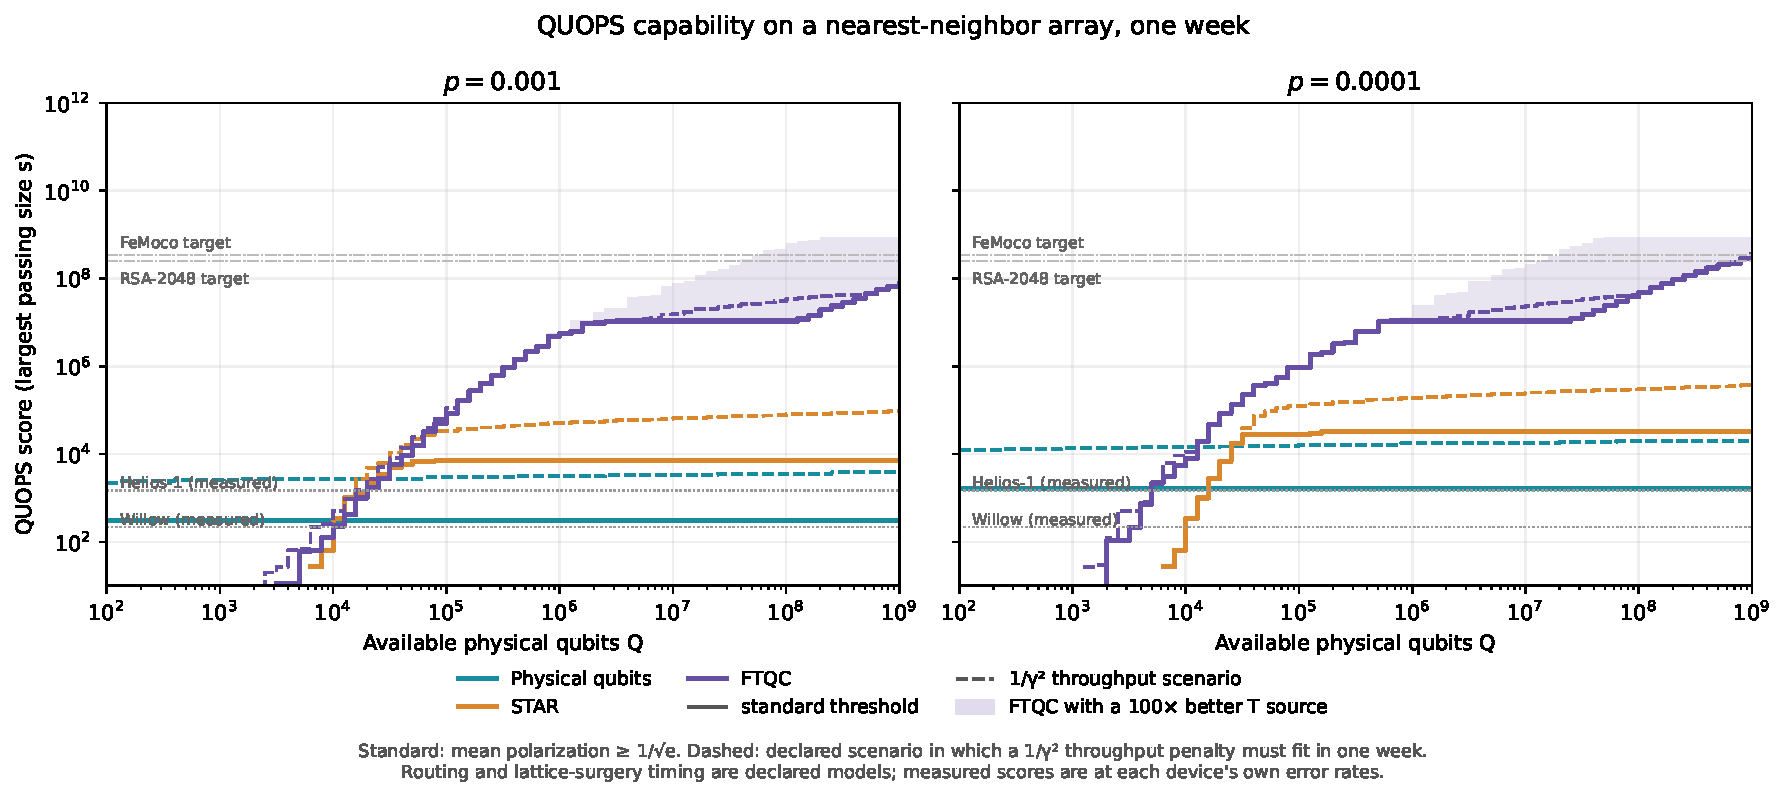
\includegraphics[width=\linewidth]{quops_capability.pdf}
\caption{QUOPS score reachable within one week versus available physical
qubits. Solid lines use the standard threshold $\bar\gamma\geq e^{-1/2}$;
dashed lines show a declared scenario in which a $1/\bar\gamma^{\,2}$ throughput
penalty must fit in the week. The shaded band gives full fault tolerance with a
T source one hundred times better. Horizontal lines give the measured Willow and Helios-1 scores, each at its
own error rates and connectivity, and the paper's RSA-2048 and FeMoco targets.
Routing is measured; lattice-surgery timing is a declared model.}\label{fig:quops}
\end{figure}

Figure~\ref{fig:quops} summarizes the first answer. Physical qubits score about
310 QUOPS at $p=10^{-3}$ however large the device, since replicas cannot raise a
polarization. STAR overtakes them with about $10^4$ qubits, briefly leads, and
then saturates near $7\times10^3$. Full fault tolerance begins last, leads from
$3\times10^4$ qubits, and scores $5.5\times10^6$ with $10^6$ qubits, about 800 times
STAR.

\begin{figure}[!htbp]
\centering
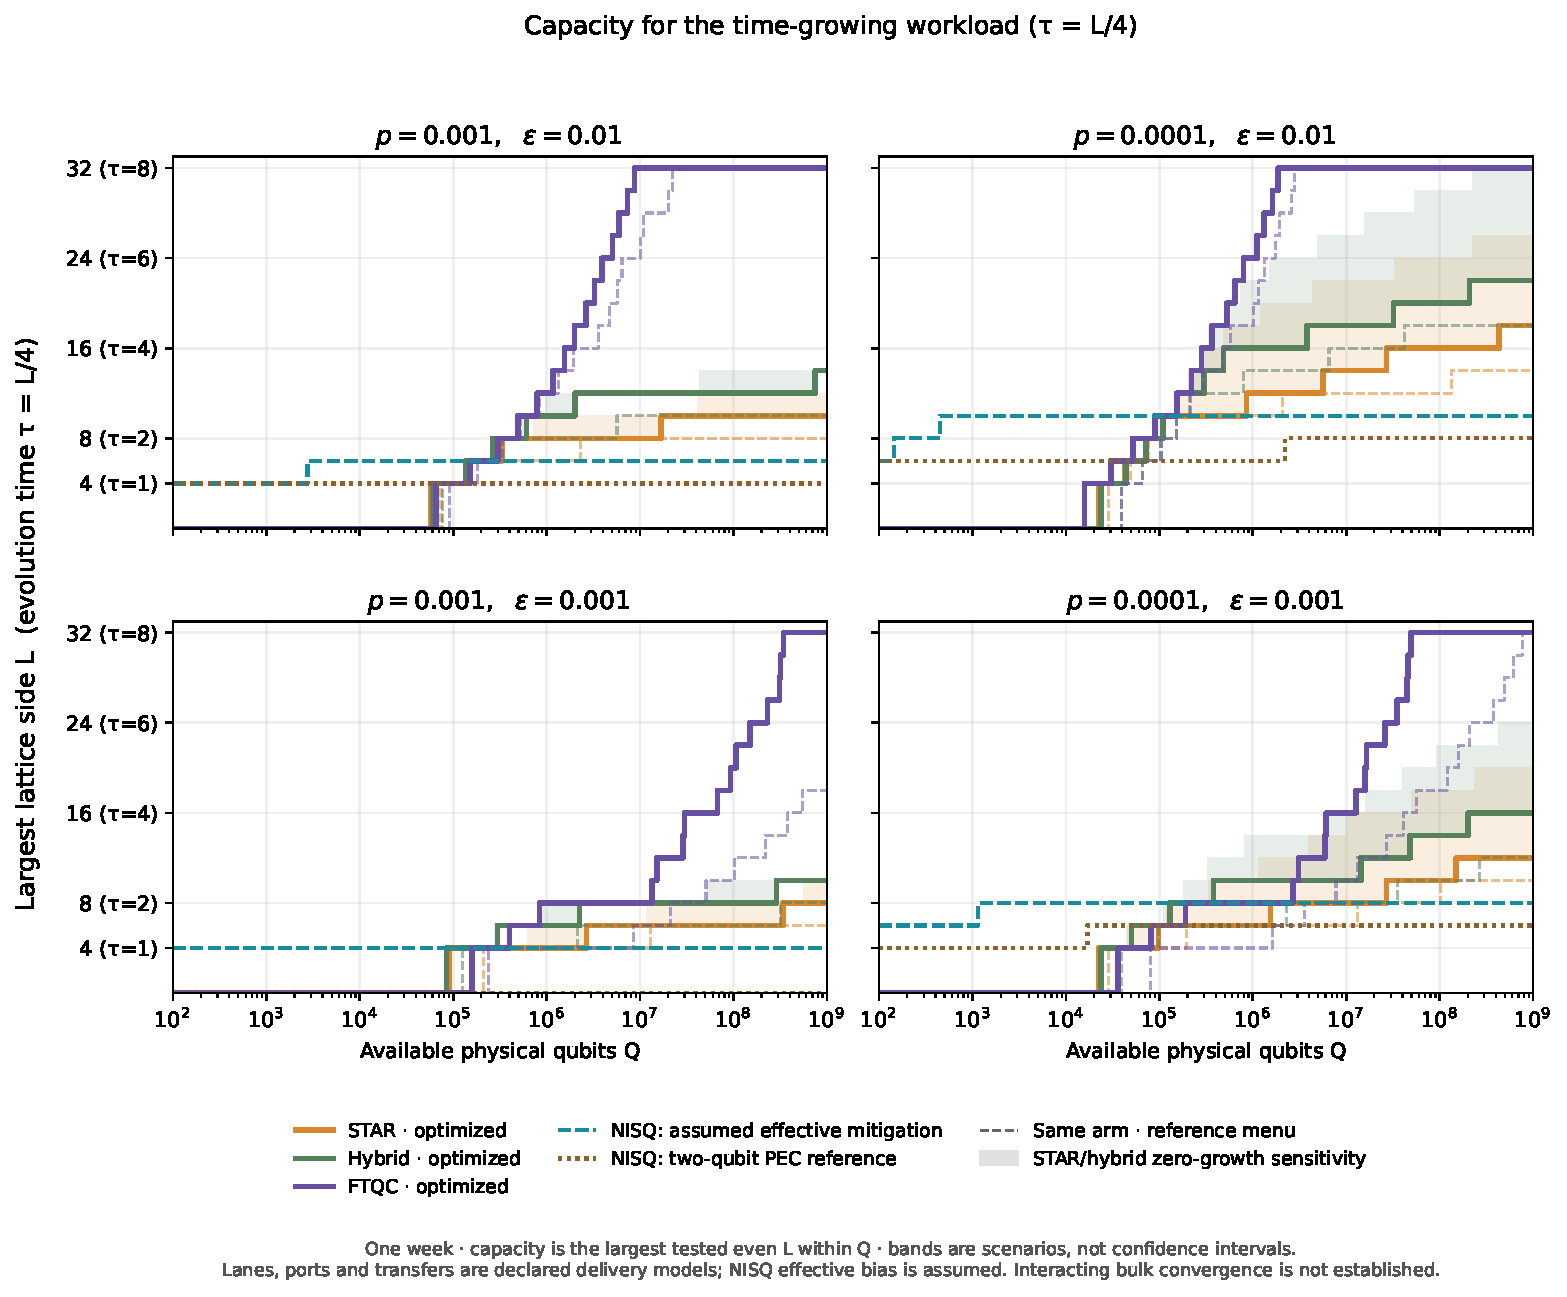
\includegraphics[width=\linewidth]{optimization_round_capacity_v2.pdf}
\caption{Largest lattice side $L$, and evolution time $\tau=L/4$, reachable
within one week as a function of available physical qubits. Solid curves use
the fully optimized model of Secs.~\ref{sec:task}--\ref{sec:architectures} with
the circuit-level surface-code law of Sec.~\ref{sec:encoded}; thin dashed
curves of the same color use the reference menu before optimization
(Sec.~\ref{sec:leader}). Bands give the STAR and hybrid zero-growth
sensitivity. NISQ curves assume an effective mitigation overhead or apply
two-qubit probabilistic error cancellation. $L=32$ is the sampled ceiling.
Delivery models are declared, not compiled, and interacting bulk convergence
is not established.}\label{fig:headline}
\end{figure}

Figure~\ref{fig:headline} gives the second. The Hubbard task is the one on which
STAR should do best, and it does: the analog arms stay within a few lattice sites
of full fault tolerance up to about $5\times10^5$ qubits and saturate at
$\tau\approx2.5$--3.5, while physical-qubit computation stops near $\tau=1.5$.
Full fault tolerance overtakes them at about $5\times10^5$ qubits and keeps
scaling to the sampled ceiling. Both orderings are consistent with one law of
the exposure variables introduced below. Physical qubits pay per gate, STAR per
radian, and full fault tolerance per synthesized rotation with only a
logarithmic precision overhead. The two workloads differ most in how fast the
radians grow, although they also differ in success criterion, connectivity
demand, and the repeated angles that full fault tolerance can batch; a
controlled sweep of the angle distribution under one criterion would test the
mechanism directly.

The remainder of this paper builds these figures from their parts.
Section~\ref{sec:task} defines both tasks and the accounting shared by all arms.
Section~\ref{sec:algorithm} describes the Trotter algorithms and the measured
step-count law for the Hubbard task. Section~\ref{sec:architectures} gives each
architecture's cost model, with calibrations collected in the appendices.
Section~\ref{sec:results} reports capabilities and crossovers for both workloads
and identifies which modeling choices move the leader. Section~\ref{sec:outlook}
states what controls the scaling, what remains conditional, and which
calculations could change the conclusions.

\begin{figure}[!htbp]
\centering
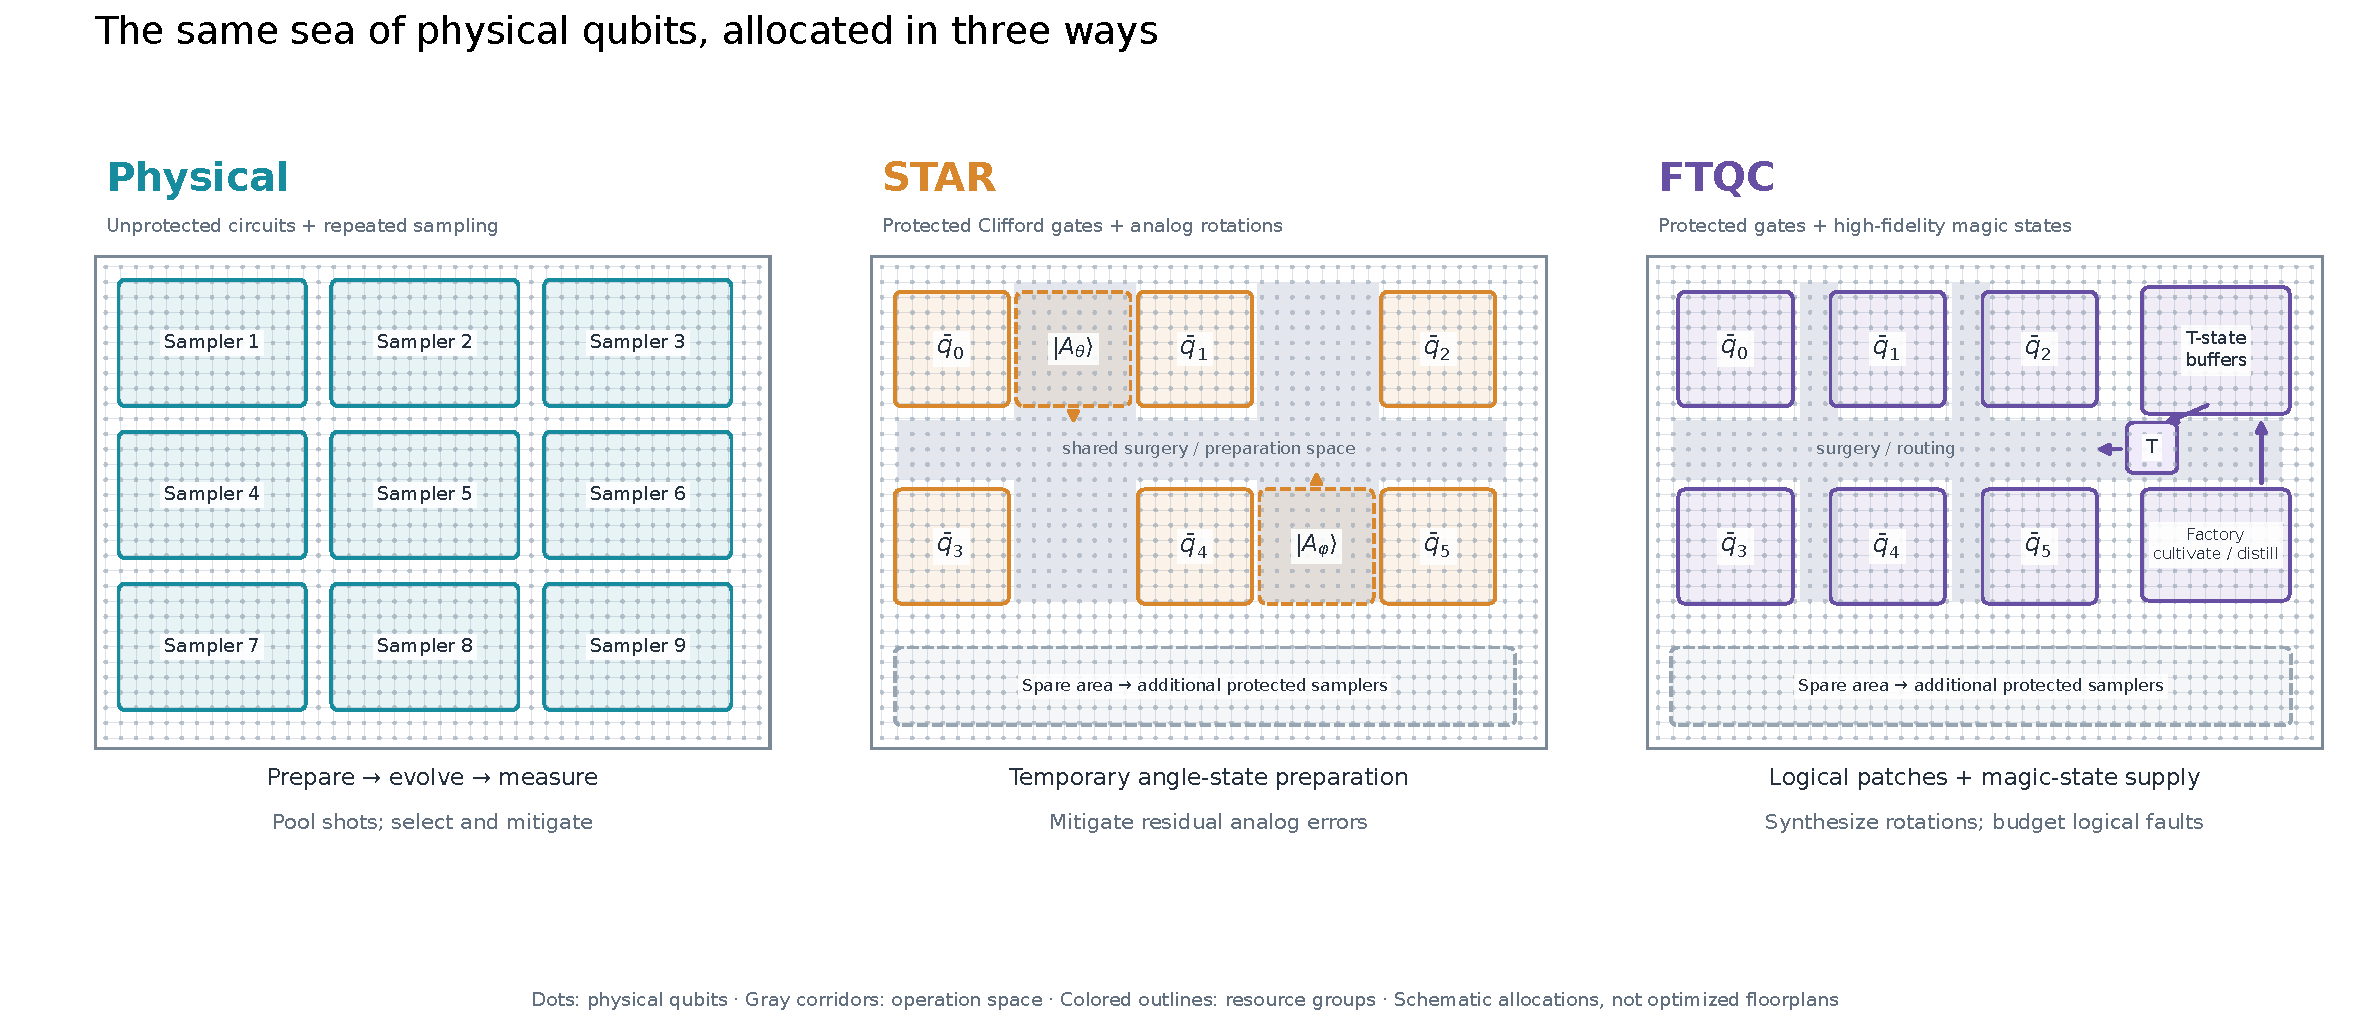
\includegraphics[width=\linewidth]{architecture_overview.pdf}
\caption{Three allocations of a common array of physical qubits. NISQ uses
many unprotected circuit replicas. STAR and FT share protected data patches
and lattice surgery. Dashed orange patches show temporary angle-state
preparation in STAR surgery ancillas~\cite{toshio}; FT supplies high-fidelity
T states to a synthesized sequence of logical operations. The drawings show
resource roles, not numerical floorplans.}\label{fig:architectures}
\end{figure}

\section{Tasks and accounting}\label{sec:task}
\subsection{Random circuits}\label{sec:quops}
A QUOPS circuit of width $w$ alternates a CNOT layer on $\lfloor w/2\rfloor$
uniformly random pairs with a layer of rotations $e^{-i\theta P/2}$, where
$P\in\{X,Y,Z\}$ and $\theta$ is uniform on $[0,2\pi)$~\cite{proctor2026quops}.
Its size $s$ counts one per rotation and two per CNOT, so a size-$s$ circuit
contains about $s/2$ rotations. A shape passes when the mean process
polarization satisfies $\bar\gamma\geq e^{-1/2}$, and the score is the largest
passing $s$ with $w^2\leq s\leq w^3$. The polarization is the product of each
operation's process infidelity $\epsilon_i$ embedded in the full register,
\begin{equation}\label{eq:quops-polarization}
 \bar\gamma\simeq\prod_i\left(1-\frac{4^w}{4^w-1}\,\epsilon_i\right),
\end{equation}
which reproduces exact noisy simulations of $w=2$--8 random circuits to 0.2\%,
whereas the product of local gate polarizations is up to 24\% pessimistic
(Appendix~\ref{app:quops}). For every shape and arm we compute the fewest
physical qubits that pass within one week, including a mirror-circuit test of
$10^4$ executions at twice the forward size; the paper prescribes no shot
count, and its experiments used $2\times10^3$--$2\times10^5$. We also show a
declared scenario in which the paper's approximate error-mitigation throughput
penalty, $1/\bar\gamma^{\,2}$, must fit in the week. It is not the sample
complexity of certifying a polarization, which would need an estimator and a
confidence calculation.

\subsection{Hubbard dynamics}
The problem has $N=L^2$ sites, $2N$ spin modes, and open boundaries. In
units of the hopping $J$,
\begin{equation}\label{eq:H}
 H/J=-\sum_{\langle ij\rangle,\sigma}
 (c^\dagger_{i\sigma}c_{j\sigma}+\mathrm{h.c.})
 +u\sum_i(n_{i\uparrow}-\tfrac12)(n_{i\downarrow}-\tfrac12),
 \qquad u=U/J=4,
\end{equation}
where the symmetric onsite form differs from $Un_\uparrow n_\downarrow$ only
by a known phase at fixed particle number. We prepare the half-filled N\'eel
product state and estimate the central doublon density
$D=\langle n_{i\uparrow}n_{i\downarrow}\rangle$ at time $\tau=Jt/\hbar$.

We tie the evolution time to the lattice, $\tau=L/4$. At fixed $\tau$, a local
observable stops depending on $L$ once the lattice contains its light cone;
for free fermions ($u=0$) the central doublon at $\tau=1$ differs from its
$L=60$ value by $2.4\times10^{-3}$ at $L=6$ and by $2.4\times10^{-4}$ at $L=8$.
A capacity measured in $L$ at fixed time therefore stops measuring physics
beyond a modest size, whereas the time-growing workload keeps the relevant
region and the lattice growing together. The fixed-time comparison is retained
as an implementation benchmark in Appendix~\ref{app:fixed-tau}. The free-fermion
numbers motivate this choice but do not bound the interacting dynamics.

\begin{table}[!htbp]
\centering
\small
\begin{tabular}{@{}ll@{}}
\toprule
Quantity & Value\\
\midrule
Connectivity & Square array, nearest neighbors\\
Gate / measurement / reset & 10 / 100 / 100~ns\\
Physical error & $p=10^{-3}$ (two-qubit), $p/10$ (one-qubit); $p=10^{-4}$ as a sensitivity\\
Syndrome cycle / feedforward & 240 / 200~ns\\
Runtime cutoff & one week, $B=604800$~s\\
Accuracy & absolute $\eps=0.01$ and $\eps=0.001$ on $D$, 95\% confidence\\
Rotation convention & $U_P(\theta)=e^{-i\theta P}$\\
\bottomrule
\end{tabular}
\caption{Fixed hardware and task parameters.}\label{tab:parameters}
\end{table}

\subsection{Accuracy contract for the Hubbard task}
The estimate must satisfy $|\widehat D-D|\leq\eps$, where the error is split
among independent contributions,
\begin{equation}\label{eq:budget}
 \eps=\eps_{\rm stat}+\eps_{\rm Trot}+\eps_{\rm bias}+\eps_{\rm inst}
 +\eps_{\rm logical}+\eps_{\rm synth}+\eps_{\rm magic},
\end{equation}
where $\eps_{\rm stat}$ is the statistical half-width, $\eps_{\rm Trot}$ the
product-formula error, $\eps_{\rm bias}$ a reserve for residual mitigation
bias ($0.1\eps$ for NISQ, STAR, and hybrid), $\eps_{\rm inst}$ the coherent
residue and retry tail of analog injection, $\eps_{\rm logical}$ the
logical-fault bias, and $\eps_{\rm synth}$ and $\eps_{\rm magic}$ the rotation
synthesis and magic-state errors. Biases are added linearly, which is
conservative. The optimizer chooses the split, together with the step count,
code distance, and delivery, separately for every arm and lattice.

\subsection{Sampling, replicas, and capacity}
Let a mitigated estimator have per-attempt variance multiplier $e^{\chi}$,
where $\chi$ is its exposure. With the doublon variance planned at
$D_*(1-D_*)$ for $D_*=0.1$, the ideal shot count and the qubits needed to
finish within the cutoff are
\begin{equation}\label{eq:sampling}
 N_0=\left\lceil\frac{z^2D_*(1-D_*)}{\eps_{\rm stat}^2}\right\rceil,\qquad
 Q_{\min}=q_a\left\lceil\frac{N_0\,e^{\chi}\,t_a}{B}\right\rceil,
\end{equation}
where $z=1.96$, $q_a$ is the area of one complete sampler, and $t_a$ its
attempt time; replicas run in parallel, and a sampler whose single attempt
exceeds $B$ is excluded. At $\eps_{\rm stat}=0.004$ this gives $N_0\approx2.2\times10^4$.
Every arm pays Eq.~\eqref{eq:sampling}; FT has $\chi=0$ but a large $q_a$.
Inverting it gives the exposure an architecture can afford,
\begin{equation}\label{eq:wall}
 \chi\lesssim\log\frac{QB}{q_aN_0t_a},
\end{equation}
so additional hardware or runtime buys exposure only logarithmically. We report
the capacity $L_{\max}(Q)$, the largest tested lattice with $Q_{\min}\leq Q$;
it is a discrete upper envelope over every even $L$ from 4 to 32 and is not
interpolated.

\section{Algorithm}\label{sec:algorithm}
\subsection{Two second-order product formulas}
Both formulas use the Jordan--Wigner encoding on a snake and drop the
single-$Z$ onsite terms, which contribute a known phase at fixed particle
number. With $E=2L(L-1)$ bonds, the remaining Hamiltonian has
\begin{equation}\label{eq:terms}
 K=4E+N=9N-8L,\qquad
 \lambda=\sum_\ell|h_\ell|=2E+\frac{|u|N}{4}=5N-4L,
\end{equation}
terms and one-norm, respectively. The termwise Strang formula applies every
term as a Pauli rotation. Merging adjacent identical rotations gives
\begin{equation}\label{eq:termwise}
 R_{\rm term}=r(2K-2)+1,\qquad \Theta_{\rm term}=\tau\lambda,
\end{equation}
where $r$ is the step count, $R$ the number of rotations, and $\Theta$ their
total angle. Notice that $\Theta$ does not depend on $r$: refining the step
multiplies the number of rotations but not their total angle. This identity
is what makes small-angle injection attractive.

Campbell's plaquette formula~\cite{campbell} partitions hopping into disjoint
four-site tiles, whose evolution needs two variable rotations and eight fixed
T gates per spin. Adapted to open boundaries with $P=L^2/4$ pink plaquettes,
$G=(L/2-1)^2$ gold plaquettes, and $B=2(L-2)$ isolated boundary bonds,
\begin{align}
 R_{\rm plaq}&=N(r+1)+4r(2P+G+B),\qquad T_{\rm fixed}=16r(2P+G),\label{eq:plaq}\\
 \Theta_{\rm dyn}&=\tau\left[\frac{|u|N}{4}+4(P+G)+2B\right].\label{eq:plaqangle}
\end{align}
At $L=4$, $\tau=1$, and $r=4$ the plaquette circuit has 288 variable rotations
of total angle 44 and 576 fixed T gates, against 889 rotations of total angle
64 for termwise Strang. STAR uses the termwise formula, since fixed $\pi/8$
rotations are expensive to inject in analog; FT and the hybrid use plaquettes.

\subsection{The step-count law}
For a local observable at fixed $\tau$, the Trotter error does not grow with
the lattice once the lattice contains the observable's causal
region~\cite{childs2021trotter}. We therefore use a law without explicit size
dependence,
\begin{equation}\label{eq:trotter}
 \eps_{\rm Trot}=\frac{C(\tau)}{r^2},\qquad r\geq8\tau,
\end{equation}
where $C(\tau)$ is 1.1 times the running maximum through $\tau$ of the measured
$|D_r-D|r^2$ over exact $2\times2$, $3\times3$, $4\times3$, and $4\times4$
dynamics. At $\tau=1$, $C=0.29$ (plaquette) and $0.21$ (termwise); by $\tau=4$
they grow to 5.8 and 3.4. The measured errors are cleanly quadratic: on the
$4\times4$ plaquette patch at $\tau=1$ they are $4.14\times10^{-3}$,
$1.03\times10^{-3}$, and $2.56\times10^{-4}$ at $r=8$, 16, and 32. The plaquette
coefficient is nearly converged across patches, 0.22--0.26 at $\tau=1$ from
$2\times2$ to $4\times4$. The termwise coefficient is not: it grows as 0.034,
0.077, 0.14, and 0.19 across the same patches. For STAR, which uses the termwise
formula, the $4\times4$ value is therefore a transferred assumption rather than
a converged one, and a larger termwise coefficient would lower its capacity.
Appendix~\ref{app:trotter} describes the matrix-free calculations, the
nested-patch checks, and the transfer to larger lattices, which remains an
assumption.

\subsection{Richardson extrapolation as an option}
Because the error is quadratic, two branches with step counts $r$ and $2r$
and coefficients $c=(-\tfrac13,\tfrac43)$ cancel its leading
term~\cite{endo2019algorithmic,low2019multiproduct}. The residual is measured
as $K_4/r^4$; on the $4\times4$ plaquette patch $|4E(2r)-E(r)|r^4/3=0.0514$ at
both $r=8$ and 16. The extrapolation is not free. Optimal allocation of shots
between branches with variance multipliers $F_i$ and attempt times $t_i$ costs
\begin{equation}\label{eq:richardson}
 T_{\rm sample}\propto\Big(\sum_i|c_i|\sqrt{F_it_i}\Big)^2,
\end{equation}
which with equal $F$ and $t_2=2t_1$ is $(\tfrac13+\tfrac43\sqrt2)^2=4.92$ times
the base branch. Branch biases add with weights $|c_i|$, so the other
allowances are divided by $\|c\|_1=5/3$. The optimizer uses it only where the
freed Trotter allowance buys more than this cost, which happens at
$\eps=0.001$.

\section{Architectures}\label{sec:architectures}
\subsection{Physical qubits with error mitigation}\label{sec:nisq}
The physical circuit is a fermionic-swap network on the nearest-neighbor
array~\cite{kivlichan2018}. We anchor its size to the published Willow
compilation of the same model at $6\times6$ and three steps~\cite{phasecraftwillow2025},
\begin{equation}\label{eq:nisq-gates}
 G=4372\,\frac{r}{3}\left(\frac{L}{6}\right)^3,\qquad
 t_a=t_{\rm reset}+294\,\frac{r}{3}\,\frac{L}{6}\,t_g+t_{\rm meas},
\end{equation}
where $G$ is the two-qubit gate count and $t_g=10$~ns; a replica occupies the
smallest square holding $2N+2$ qubits. Two estimators bracket the arm. The
reference is two-qubit probabilistic error cancellation (PEC), whose
depolarizing inverse has $\gamma_2=1+2p/s_2$ per gate with $s_2=1-16p/15$,
so that $\chi_{\rm PEC}=2G\log\gamma_2\simeq4pG$. The second line assumes an
effective mitigation overhead $\chi_{\rm eff}=\kappa pG$ with $\kappa=1.05$,
chosen so that the Willow circuit costs a factor 100 in variance; it is not
fitted. Measured attenuation in the Phasecraft and Willow data points to
$\kappa\approx0.2$--0.4, but neither experiment establishes our absolute
accuracy with controlled bias. For this reason we also solve the inverse
problem: the variance and remaining offset that any physical estimator would
need to match the encoded arms (Appendix~\ref{app:nisq}).

The physical arm meets its wall abruptly. Holding the Trotter error at a fixed
absolute accuracy needs about eight steps per unit time, so $r\propto\tau\propto L$
and $G\propto rL^3$ give an exposure $\chi\propto L^4$ for the time-growing
workload, while Eq.~\eqref{eq:wall} lets the affordable exposure grow only as
$\log Q$. The capacity therefore scales as $L_{\max}\propto(\log Q)^{1/4}$.
Under the assumed effective overhead at $p=10^{-3}$ and $\eps=0.01$, $L=6$
($\tau=1.5$, twelve steps, $1.7\times10^4$ gates) needs about $3\times10^3$ qubits,
while $L=8$ ($\tau=2$) needs $10^{21}$; six decades of hardware buy about 20\% in
lattice side. The published Willow experiment reached $6\times6$ with one to
three Trotter steps and at most 4372 two-qubit gates~\cite{phasecraftwillow2025}.
At $4\times4$ and three steps its processed local doublon matches continuous
interacting dynamics to 0.0103 RMS, at our accuracy target (Sec.~\ref{sec:external});
a $6\times6$ lattice at $\tau=1.5$ and $\eps=0.01$ needs four times their largest
circuit.

For random circuits the physical arm must also route arbitrary pairs on the
nearest-neighbor array. We use laws measured on 900 routed QUOPS circuits of
widths 4--144 (Appendix~\ref{app:quops}): about $0.35w^{1.59}$ fused two-qubit
gates per layer with Cirq's router, or depth growing only as $w^{0.62}$ with a
constructive sorting network, whichever loses less polarization at each width.
The noise is the convention of the surface-code calibration: two-qubit
depolarizing error $p$ per gate, one-qubit error $p/10$, and one-qubit error $p$
per idle 10~ns slot, each entering Eq.~\eqref{eq:quops-polarization} with process
infidelity equal to its total Pauli error probability. Without mitigation,
replicas only shorten the mirror test.

\subsection{Encoded protection}\label{sec:encoded}
STAR, FT, and the hybrid store logical qubits in surface-code patches of
$2d^2$ physical qubits and perform Clifford operations by lattice surgery.
Each patch fails per syndrome round with probability
\begin{equation}\label{eq:logical}
 p_L(d)=A\,\Lambda^{-(d+1)/2},\qquad \Lambda=p_{\rm th}/p.
\end{equation}
A circuit-level memory calibration under our noise model and 240~ns schedule,
using Stim and PyMatching~\cite{gidney2021stim,higgott2023sparse} with
$9.6\times10^7$ shots at $d=3$--9, gives $\Lambda=7.41$ (95\% interval
7.20--7.62) and $A=0.077$ at $p=10^{-3}$, and $\Lambda=89$ with a wide interval
at $p=10^{-4}$ (Appendix~\ref{app:surface}). The widely used reference
$A=0.1$, $\Lambda=10$ is optimistic by 4--6 in code distance at the operating
points of this study. The same law serves every encoded arm, so it favors none
of them against the others.

For $V$ patch-rounds per attempt, the logical-fault bias is at most $Vp_L(d)$.
Under PEC of the analog rotations, a fault's bias can be amplified by up to
$e^{\chi/2}$, so the smallest admissible distance satisfies
\begin{equation}\label{eq:distance}
 V\,p_L(d)\leq\eps_{\rm logical}\,e^{-\chi/2}.
\end{equation}
Because $V$ itself depends on $d$ through the attempt time, the distance is
found self-consistently. Faults are budgeted per attempt; the campaign is not
required to contain zero logical faults. On random circuits, each layer of
long-range CNOTs is assumed to take two code clocks of lattice surgery in the
fast data block without congestion, a declared model.

\subsection{STAR}\label{sec:star}
\begin{figure}[!htbp]
\centering
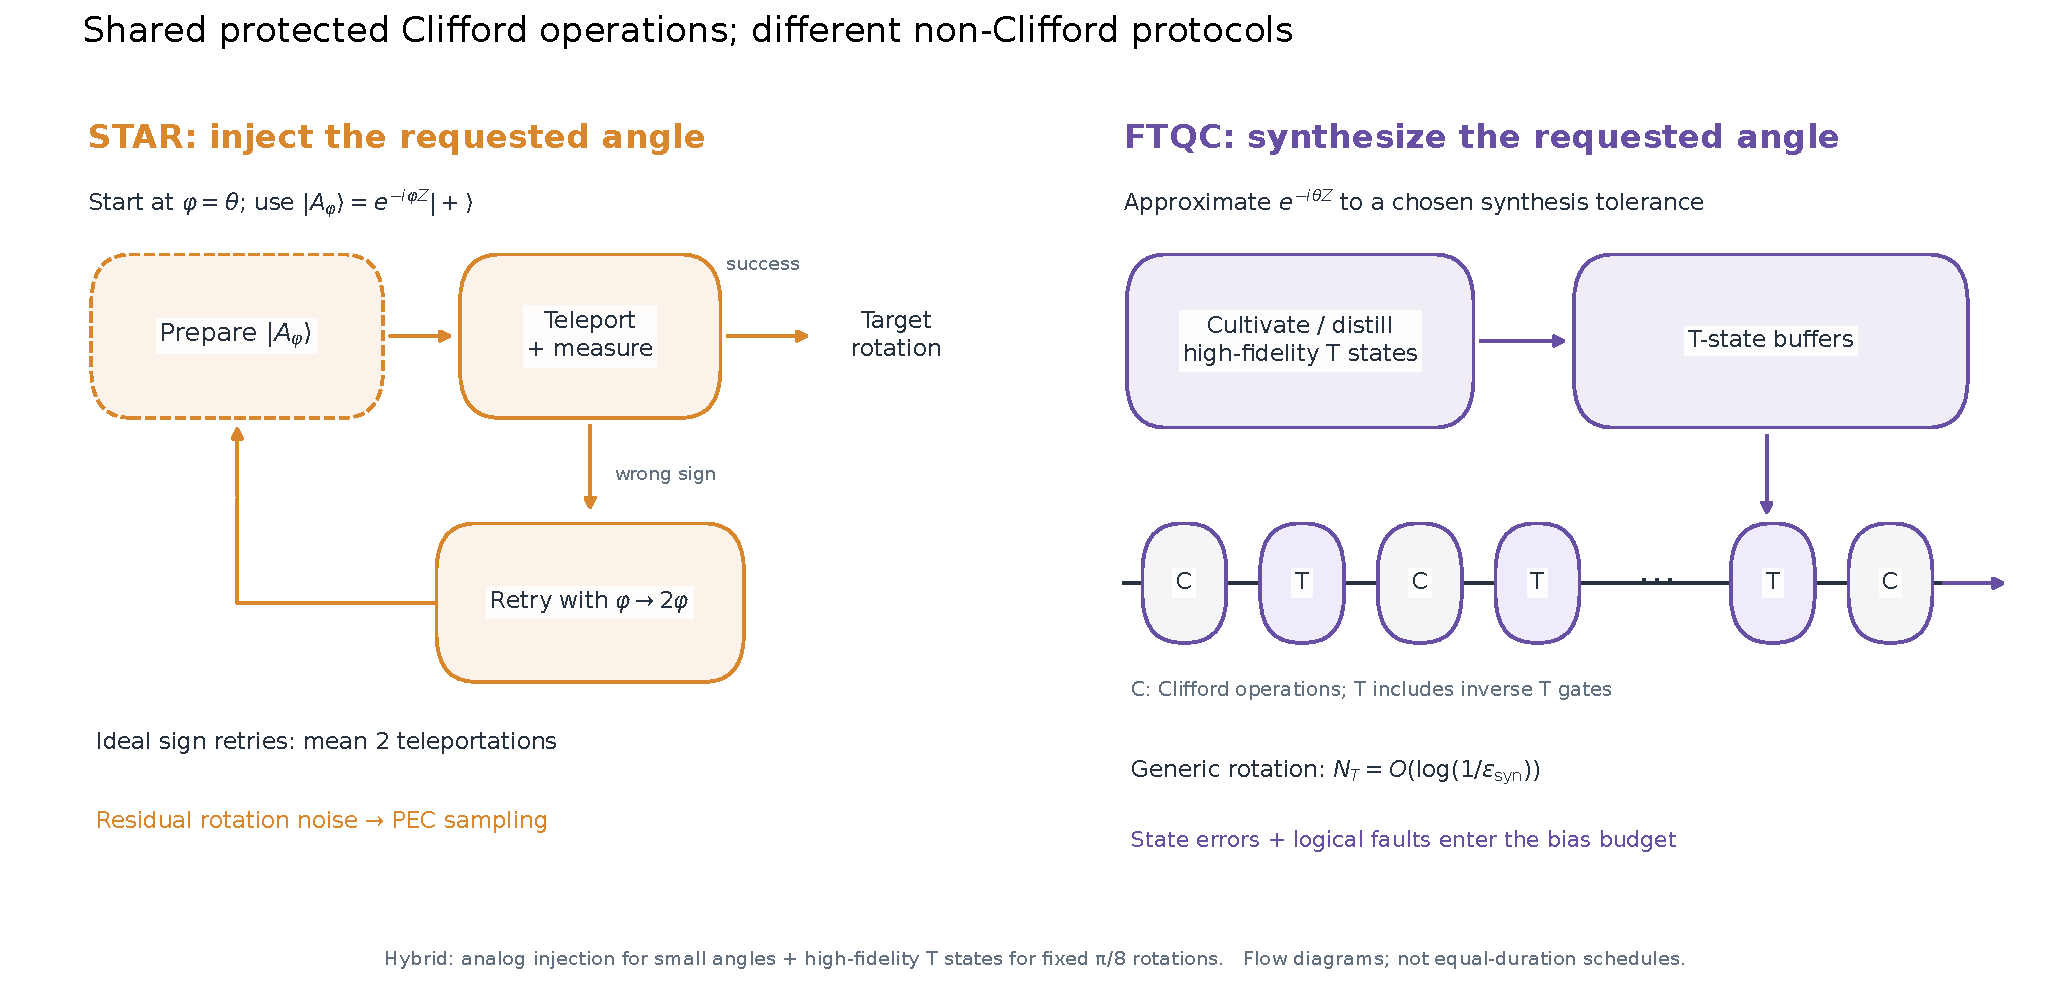
\includegraphics[width=\linewidth]{rotation_protocols.pdf}
\caption{Two implementations of the same target rotation, in the convention
$e^{-i\theta Z}$. STAR prepares an angle-specific resource state and uses
teleportation with angle-doubling corrections~\cite{akahoshi,toshio}.
Ideal sign outcomes require two teleportations on average; this does not
include rejected preparation attempts or their cost. FTQC consumes
high-fidelity T states in a Clifford+T approximation, whose generic T count
grows logarithmically with inverse synthesis tolerance~\cite{ross}. The
hybrid chooses between these paths by operation class. These are protocol
flows, not schedules with equal durations or calibrated factory footprints.}
\label{fig:rotation-protocols}
\end{figure}

STAR teleports each rotation from an angle-specific resource state. A failed
teleportation applies the rotation with the opposite sign and is corrected by
injecting twice the angle, repeating until success (RUS)~\cite{akahoshi,toshio};
Figure~\ref{fig:rotation-protocols} shows the protocol. We evaluate the
transversal multi-rotation preparation of Ref.~\cite{toshio} exactly at every
workload angle: a $k=(d_i+1)/2$ factor preparation at injection distance $d_i$
has undetected generator faults with probability $p/15$ per pair factor and
$p/30$ for the final factor, which fixes both the preparation acceptance and
the accepted channel. The resulting rotation multiplies off-diagonal elements
by $c_j$, and PEC of its dephasing costs
\begin{equation}\label{eq:star}
 \chi_{\rm STAR}=-2\sum_j\log(\operatorname{Re}c_j)
 \simeq4\alpha p\,\Theta_{\rm term},
\end{equation}
where the sum runs over rotations with multiplicity and $\alpha$, of order
1--3, is an effective prefactor that depends on angle and injection distance. The
coherent residue $|\operatorname{Im}c_j|$ and the finite RUS tail are charged to
$\eps_{\rm inst}$. Injection seeds $d_i=5$, 9, and 25 grow to receivers of
distance 13 or 25. Their growth error is the upper limit from $2.4\times10^7$
decoded growth shots, composed as an independent channel; most campaigns
observed no failures, so this is a bound rather than a measured rate
(Appendix~\ref{app:star}).

Two refinements of the protocol are options of the optimizer. Probabilistic
coherent error cancellation (PCEC) removes the coherent part of each trial and
roughly doubles its dephasing~\cite{toshio}. Without it, averaging over RUS
branches already cancels the coherent term at first order in our instrument,
halving the exposure; Toshio \textit{et al.} report the opposite ordering for
the branch-averaged channel, and we have not reconciled the two
(Appendix~\ref{app:raw-rus}). Rotations can also be injected in parallel
lanes. Each lane occupies six tiles; disjoint Jordan--Wigner supports limit
concurrent termwise rotations to at most $L$; and more than four lanes use the
fast data block. The attempt time is the analog service time divided by the
number of lanes, plus surgery and handoff. For random circuits the injected
angle is $\theta/2$ reduced modulo $\pi/4$ by Clifford corrections, which is
uniform on $[-\pi/8,\pi/8]$; we average the instrument over that distribution.
Its mean magnitude, $\pi/16$, is roughly seven times the Trotter angles of the
Hubbard task.

\subsection{Full fault tolerance}\label{sec:ft}
FT synthesizes each variable rotation to operator error $\zeta$ with
\begin{equation}\label{eq:synthesis}
 n_T=\left\lceil3.02\log_2(1/\zeta)+0.77\right\rceil,\qquad
 \zeta=\frac{\eps_{\rm synth}}{2R},
\end{equation}
T gates~\cite{ross}. Because the plaquette angles are shared by every tile of
a stage, Hamming-weight phasing can replace a batch of $b$ equal rotations by
$\lfloor\log_2b\rfloor+1$ rotations and $b-\mathrm{popcount}(b)$ Toffolis,
with that workspace charged~\cite{campbell}. Magic states come from
cultivation~\cite{gidney2024cultivation}: 1024 qubits and about 100 cycles per
state at error $2\times10^{-9}$, with an optional 15-to-1 cleanup stage of
twelve tiles and output error $35q^3$. Each factory costs $1024+2d^2$ qubits,
or $1024+13\cdot2d^2$ with cleanup.

Supply and consumption run concurrently. A synthesized rotation is a serial T
sequence, whereas the rotations of one plaquette stage are independent, so
with $P$ consumption ports the serial T depth is
\begin{equation}\label{eq:serial-t}
 N_T^{\rm serial}=n_T\sum_s m_s\left\lceil\frac{R_s}{P}\right\rceil
 +\frac{N_T-n_TR}{P},
\end{equation}
where stage $s$ is repeated $m_s$ times with $R_s$ synthesized rotations and
$N_T$ is the total T count. With $F$ factories of service time $s_F$, the
attempt time is
\begin{equation}\label{eq:ft-time}
 t_a=\Big[2d+\max\Big(d\big(c_TN_T^{\rm serial}+W/P\big),\ \lceil N_T/F\rceil s_F\Big)\Big]t_c
 +N_T^{\rm serial}t_{\rm ff}+t_{\rm reset}+t_{\rm meas},
\end{equation}
where $c_T$ is 9 clocks per T for the compact block with one port and one
clock for the fast block, $W$ counts two Clifford clocks per rotation and per
Toffoli, $t_c=240$~ns, and $t_{\rm ff}$ is the feedforward latency. The optimizer chooses block, ports, factories, batch size, cleanup,
and distance together; each extra port costs two tiles. The cultivated state
is transferred from its distance-15 patch into the data distance at a cost of
$2\max(d,15)$ cycles, so the data distance may be smaller than 15. For random
circuits we follow the paper and charge each synthesized rotation its squared
diamond-distance error, $\zeta^2$, in Eq.~\eqref{eq:quops-polarization}; random
angles admit no Hamming-weight batching.

\subsection{The hybrid}\label{sec:hybrid}
The hybrid runs the plaquette circuit, injects its variable rotations as in
STAR, and draws its fixed $\pi/8$ rotations from the FT cultivation supply.
It therefore pays STAR's exposure only on $\Theta_{\rm dyn}$ of
Eq.~\eqref{eq:plaqangle}, without synthesizing any rotation, at the cost of
factory area and a magic-state error amplified by $e^{\chi/2}$. A proposed
extra protection step pays at fixed shot budget when
\begin{equation}\label{eq:hybrid}
 \Delta\log t_a+\Delta\chi-\Delta\log m<0,
\end{equation}
where $m$ is the number of replicas; the hybrid is the simplest instance of
this operation-dependent protection.

\section{Results}\label{sec:results}
\subsection{Random circuits}\label{sec:quops-results}
Figure~\ref{fig:quops} shows the capability of each arm on random circuits. At $p=10^{-3}$ and under the standard threshold,
physical-qubit computation scores about 310 whatever the device size, since
extra replicas cannot raise a polarization. A reimplementation by another
workshop group obtains about 150 at the same $p$; the difference comes from our
routing, measured on 900 circuits rather than modeled, and from the embedded
polarization product. Willow measured 216 at its own, somewhat higher error
rates. STAR overtakes the physical arm at $10^4$ qubits and leads alone between
$10^4$ and $2.5\times10^4$, where full fault tolerance is still limited by its
fixed area, but saturates at $7\times10^3$, because each random rotation injects
an angle of average magnitude $\pi/16$, roughly seven times the Trotter angles
of the Hubbard task. Full fault tolerance leads for good
from $3\times10^4$ qubits, reaches $10^4$ QUOPS with $5\times10^4$ qubits, and
scores $5.5\times10^6$ at $10^6$ qubits, about 800 times STAR. On the Hubbard
task, by contrast, the analog arms stayed within a few lattice sites of full
fault tolerance up to about $5\times10^5$ qubits. The difference is the one the
exposure picture predicts: STAR pays per radian, and here the radians are
large.

Full fault tolerance then plateaus near $1.1\times10^7$ from about $3\times10^6$
to $10^8$ qubits. Beyond that size a circuit needs more than about $2\times10^8$
T states, which exceeds what cultivated states of error $2\times10^{-9}$ can
supply within the polarization budget, and every factory must add a 15-to-1
cleanup stage that is roughly seven times larger and fifteen times slower. At
$10^9$ qubits the score reaches $7.5\times10^7$, short of the paper's RSA-2048
and FeMoco targets of $2.5$--$3.4\times10^8$; at $p=10^{-4}$ it reaches them with
about $8\times10^8$ qubits. The plateau is a feature of source quality, not of
full fault tolerance: with a declared T source one hundred times better, the
same model reaches the RSA-2048 target with $4\times10^7$ qubits at $p=10^{-3}$.
Under the $1/\bar\gamma^{\,2}$ throughput scenario the physical arm reaches about
$4\times10^3$ and STAR about $10^5$ at $10^9$ qubits, without changing the
ordering. The mirror test's shot count matters only where logical shots are
slow: with Willow's $2\times10^5$ executions instead of $10^4$, full fault
tolerance beyond $s\approx10^7$ needs roughly an order of magnitude more qubits.

For the shapes of the paper's planar projection, our full fault tolerance needs
4--7 times more physical qubits than reported there, for example $3.9\times10^4$
rather than $10^4$ for $w=21$ and $s=9240$. Our calibrated $\Lambda=7.41$ raises
the code distance relative to a uniform-depolarizing law, and the fast data
block and 1024-qubit cultivation sources add area; we report the ratio rather
than tune toward it.

\subsection{Hubbard capacity and crossovers}\label{sec:capacity}
Figure~\ref{fig:headline} and Table~\ref{tab:crossovers} give the capacity of
each arm for the time-growing Hubbard workload. At $p=10^{-3}$ and $\eps=0.01$,
physical-qubit computation reaches $L=6$ ($\tau=1.5$) with about
$3\times10^3$ qubits and stops there. Encoded computation overtakes it at about
$2.7\times10^5$ physical qubits. Full fault tolerance leads alone beyond
$5\times10^5$ qubits and reaches the $\tau=8$ ceiling at $9\times10^6$, while STAR
saturates at $L=10$ ($\tau=2.5$) and the hybrid at $L=14$ ($\tau=3.5$).
Tightening the accuracy to $\eps=0.001$ moves the point beyond which full
fault tolerance leads to $8.4\times10^5$ qubits, and reaching the ceiling then
takes $3.5\times10^8$ qubits. At $p=10^{-4}$ every arm reaches further: the
analog arms saturate at $\tau=4.5$--5.5 for $\eps=0.01$, and full fault
tolerance reaches the ceiling at $1.9\times10^6$ qubits.

\begin{table}[!htbp]
\centering
\small
\begin{tabular}{@{}rrrrrr@{}}
\toprule
$p$ & $\eps$ & Encoded $>$ NISQ (PEC / eff.) & FT ahead to stay & STAR / hybrid & FT at $\tau=8$\\
\midrule
$10^{-3}$ & $0.01$ & $1.4\times10^5$ / $2.7\times10^5$ & $5.0\times10^5$ & $\tau=2.5$ / 3.5 & $8.7\times10^6$\\
$10^{-3}$ & $0.001$ & $0.9\times10^5$ / $3.0\times10^5$ & $8.4\times10^5$ & $\tau=2$ / 2.5 & $3.5\times10^8$\\
$10^{-4}$ & $0.01$ & $0.5\times10^5$ / $1.5\times10^5$ & $2.2\times10^5$ & $\tau=4.5$ / 5.5 & $1.9\times10^6$\\
$10^{-4}$ & $0.001$ & $1.3\times10^5$ / $3.8\times10^5$ & $3.1\times10^6$ & $\tau=3$ / 4 & $5.0\times10^7$\\
\bottomrule
\end{tabular}
\caption{Physical qubits at which each transition occurs for the time-growing
workload, with all optimizer options and the calibrated surface-code law.
``Encoded $>$ NISQ'' compares with two-qubit PEC, which has a bound behind it,
and with the assumed effective mitigation line. ``FT ahead to stay'' is the
point beyond which no analog arm exceeds FT at any larger budget; ties are
allowed. ``STAR / hybrid'' gives the evolution time at which each saturates. Lattices are
every even $L$ from 4 to 32, and budgets are sampled on a logarithmic grid.}\label{tab:crossovers}
\end{table}

For the time-growing workload, full fault tolerance leads alone in every cell
with at least $10^8$ qubits. Below that, the hybrid holds a narrow window: it
ties full fault tolerance at $p=10^{-3}$, $\eps=0.001$, and $10^7$ qubits, and
leads alone at $p=10^{-4}$, $\eps=0.001$, and $10^6$ qubits. STAR never leads
alone once its delivery and injection options are optimized, and the hybrid
never falls below it.

\subsection{External checks}\label{sec:external}
Two published operating points check the accounting from outside. For the
encoded arms, we replayed the TopQAD resource ledger for Hubbard ground-state
energy estimation~\cite{chung}. All 16 STAR footprints reproduce the published
values, 14 of 16 runtimes without PEC agree within 2.3\%, and all 16
time-optimal FT entries agree within 2.8\%; the two remaining STAR rows are
internally inconsistent in the publication. For physical qubits, we reconstructed
the Willow $4\times4$, $U=4$ circuits~\cite{phasecraftwillow2025,willowdata2025} and
computed ideal-circuit and continuous interacting references at all 24 saved
times (Fig.~\ref{fig:willow-matched}). The processed experimental local doublon
differs from continuous dynamics by 0.0103 RMS at three Trotter steps, with 71\%
of points within 0.01. The two contributions respond oppositely to refinement:
from one to three steps the ideal circuit's error falls from 0.045 to 0.013,
while the processed data's discrepancy from the ideal circuit grows from 0.0047
to 0.0095. This is the trade-off behind the physical-qubit wall. Refinement buys
algorithmic accuracy with circuit exposure, and at three steps the total also
benefits from partial cancellation between the two, which a controlled error
budget cannot credit.

\begin{figure}[!htbp]
\centering
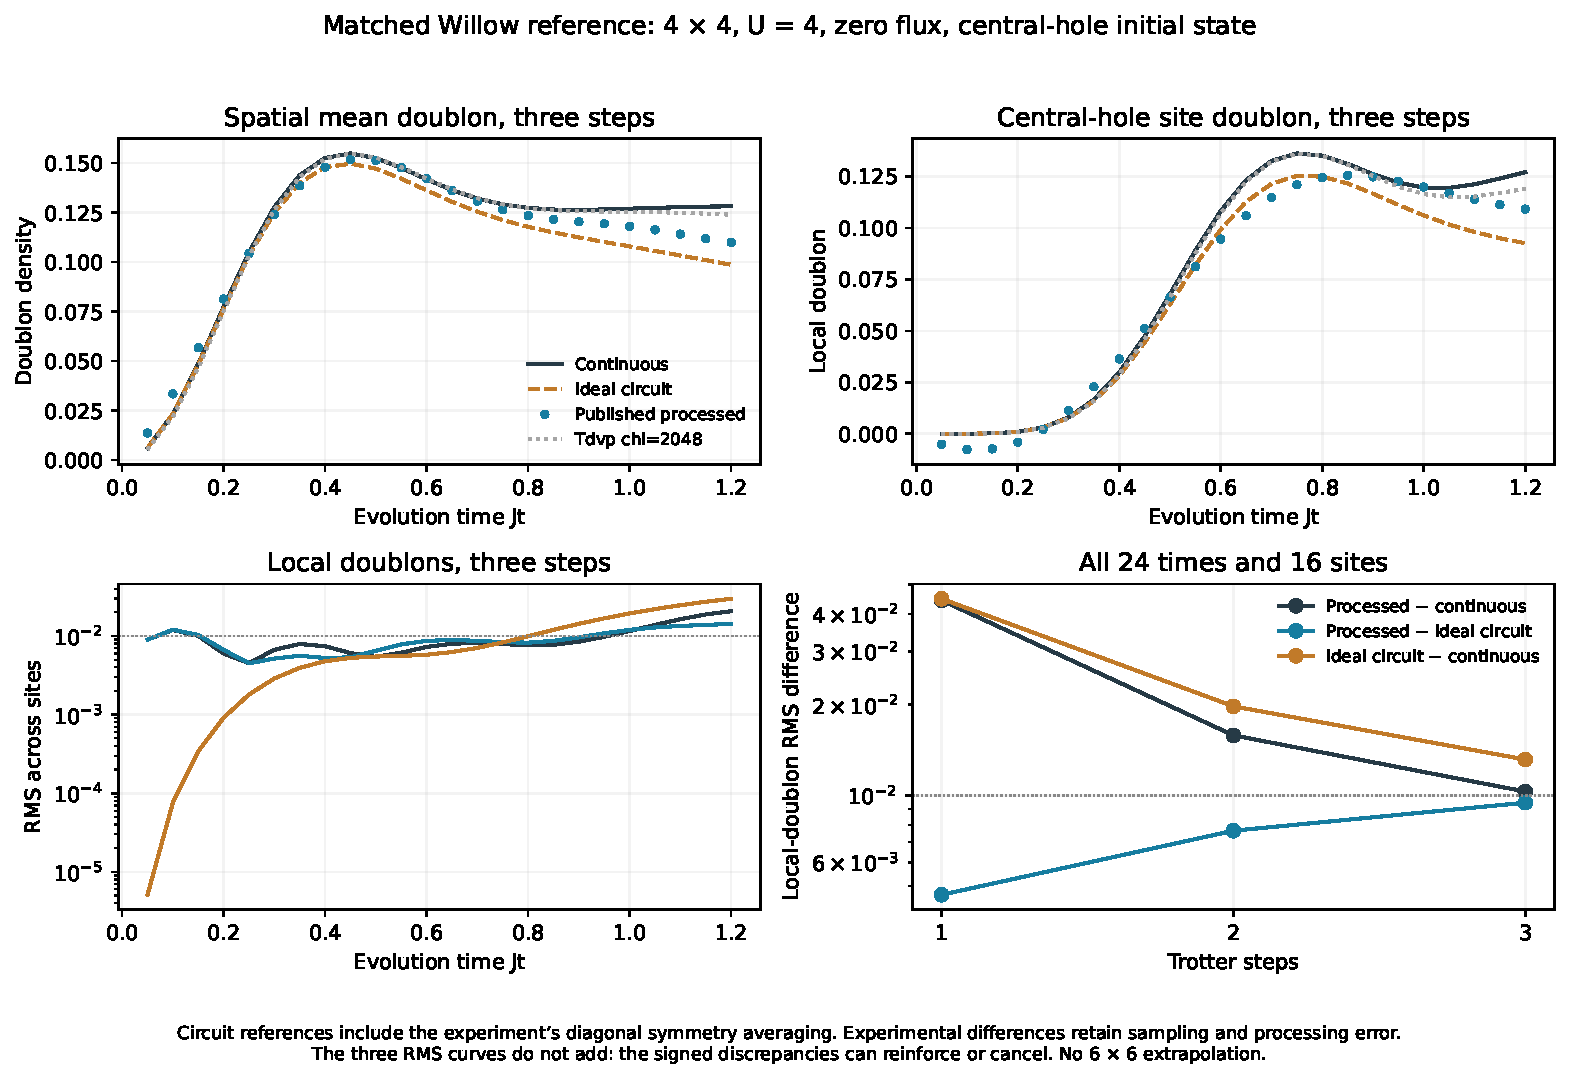
\includegraphics[width=\linewidth]{willow_matched_reference.pdf}
\caption{Willow $4\times4$, $U=4$ data against matched references. Processed
experimental estimates are compared with ideal circuits of the same step count
and with continuous interacting dynamics; the decomposition separates circuit
(Trotter) error from observed experimental discrepancy. Details are in the
Supplementary Material.}\label{fig:willow-matched}
\end{figure}

\subsection{Which choices move the leader}\label{sec:leader}\label{sec:optimization-round}
The model contains choices that a simpler comparison would fix in advance:
four analog lanes, one T-consumption port with Hamming-weight batches of at
most 16, a data distance no smaller than the cultivation output distance,
noisy PCEC for every analog rotation, and a single Trotter branch. We tested
each alternative alone and all together against this reference menu, which
reproduces our earlier integrated model in 335 of 336 replayed cases to
$10^{-9}$ in $\log_{10}Q$; the remaining case, a STAR design at $10^{78.7}$
qubits, lies beyond an exposure cutoff that cannot affect capacity below
$10^9$ qubits. Figure~\ref{fig:leaders} and Table~\ref{tab:leader-changes}
attribute the changes.

\begin{figure}[!htbp]
\centering
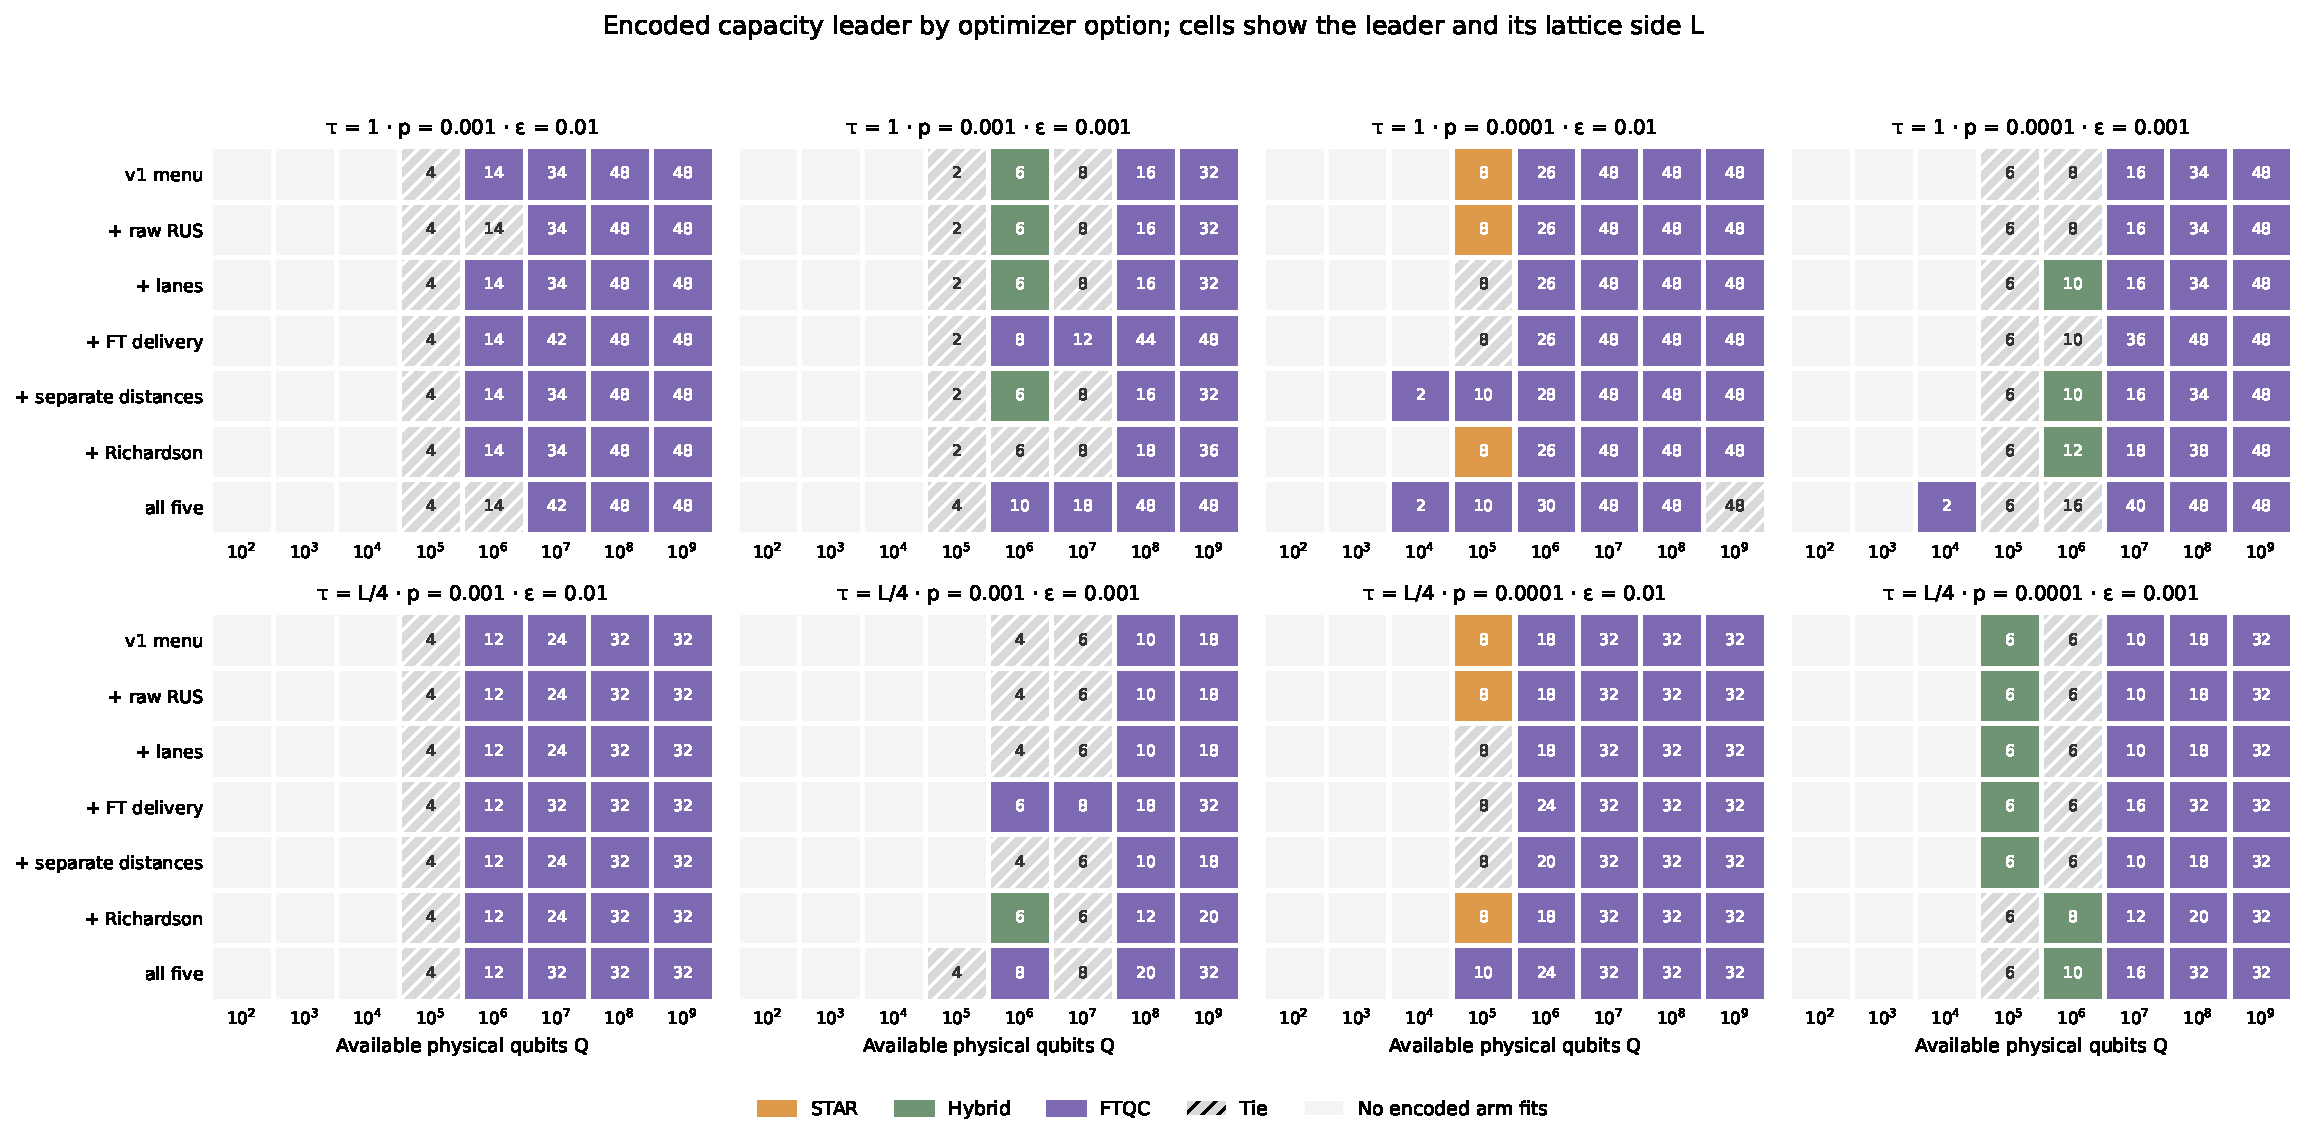
\includegraphics[width=\linewidth]{optimization_round_leaders_v2.pdf}
\caption{Encoded capacity leader for each configuration (rows), qubit budget
(columns), time family, physical error, and precision, with the calibrated
surface-code law. Numbers give the leader's lattice side; hatched cells are
ties. The reference menu is the top row of each panel.}\label{fig:leaders}
\end{figure}

\begin{table}[!htbp]
\centering
\small
\begin{tabular}{@{}lrp{0.62\linewidth}@{}}
\toprule
Option & Cells & Mechanism\\
\midrule
FT delivery & 8 & Larger Hamming-weight batches cut synthesized rotations; ports and factories cut the attempt time\\
Richardson & 6 & Base step count $8\tau$ with a $K_4/r^4$ residual frees the Trotter allowance, all at $\eps=0.001$\\
Separate distances & 4 & FT and hybrid run below $d=15$ at $p=10^{-4}$\\
Lanes & 3 & Parallel analog injection, mainly for the hybrid\\
Raw RUS & 2 & Lower analog exposure within the restricted instrument\\
All five & 15 & Mostly earlier separation of full fault tolerance\\
\bottomrule
\end{tabular}
\caption{Cells, out of 64, in which each option alters the encoded capacity
leader relative to the reference menu.}\label{tab:leader-changes}
\end{table}

Joint T delivery moves the leader most often. At $48\times48$, $\tau=1$, and
$\eps=0.001$, whole-group phasing reduces the T count from $1.45\times10^7$ to
$3.0\times10^6$, while 32 ports and 1024 factories reduce the attempt time from
135~s to 2.1~s; the required area falls from $10^{9.6}$ to $10^{8.1}$ qubits,
although factories occupy 54\% of it. Separate source and data distances, or
optimized lanes, remove the only cell in which STAR led alone ($p=10^{-4}$,
$\eps=0.01$, $Q=10^5$). Raw RUS rarely moves the leader but supplies most of
the analog gain; $16\times16$ STAR at $\tau=1$ and $\eps=0.01$ falls from
$10^{10.3}$ to $10^{8.2}$ qubits with it alone. That gain rests on a coherent
cancellation which the branch-averaged analysis of Ref.~\cite{toshio} does not
reproduce (Appendix~\ref{app:raw-rus}); the conclusions about full fault
tolerance do not depend on it.

\subsection{Sensitivity to the surface-code law}\label{sec:law-sensitivity}
Replacing the reference law ($A=0.1$, $\Lambda=10$) by the calibrated one
raises the code distance of every encoded arm by two at small lattices and
by up to six at the largest, and delays each transition modestly
(Table~\ref{tab:law-sensitivity}). The effect is largest at $p=10^{-3}$, where
the calibrated $\Lambda=7.41$ departs most from the reference, and small at
$p=10^{-4}$. Because the arms protect different volumes, a shared law need not
move them equally: it changes the encoded leader in 4 of 64 cells, all at fixed
$\tau=1$. At strict precision and $10^6$ qubits, for example, the hybrid and full
fault tolerance tie at $L=10$ under the reference law, while the calibrated law
leaves the hybrid at $L=8$. On the time-growing workload no leader changes.

\begin{table}[!htbp]
\centering
\small
\begin{tabular}{@{}rrrr@{}}
\toprule
$p$ & $\eps$ & Encoded beats NISQ & FT at $\tau=8$\\
\midrule
$10^{-3}$ & $0.01$ & $1.9\to2.7\times10^5$ & $7.0\to8.7\times10^6$\\
$10^{-3}$ & $0.001$ & $2.2\to3.0\times10^5$ & $2.4\to3.5\times10^8$\\
$10^{-4}$ & $0.01$ & $1.2\to1.5\times10^5$ & $1.8\to1.9\times10^6$\\
$10^{-4}$ & $0.001$ & $3.8\to3.8\times10^5$ & $5.0\to5.0\times10^7$\\
\bottomrule
\end{tabular}
\caption{Physical qubits at two transitions under the reference and the
calibrated surface-code law, with all optimizer options.}\label{tab:law-sensitivity}
\end{table}

\section{Discussion}\label{sec:outlook}
The exposure variables explain the ordering. With local full-lattice
compilation, the number of rotations is $R=O(Nr)$ and their total angle is
$\Theta=O(N\tau)$. Physical PEC therefore has exponent $O(pNr)$, and STAR's
small-angle exposure $O(pN\tau)$, which the time-growing workload makes
$O(pL^3)$; injection floors, growth, and the fixed plaquette angles restore
some growth with $r$. Full fault tolerance instead needs $O(Nr\log(Nr/\eps))$
T states and a code distance logarithmic in the protected volume, at the price
of a large starting area. Every arm has the logarithmic sampling allowance of
Eq.~\eqref{eq:wall}. An exponent that grows as a power of the lattice
therefore meets a wall, and only full fault tolerance, whose sampling exponent
is zero, keeps scaling. The two workloads isolate the per-radian term. With
rotations of order one, STAR falls three orders of magnitude behind full fault
tolerance at $10^6$ qubits; with small Trotter angles it stays within a few
lattice sites until about $5\times10^5$ qubits.

Several limitations remain. Lane, port, and transfer charges are declared
rather than compiled. The Trotter law is measured only through $4\times4$
patches and is transferred beyond $\tau=4$, and interacting bulk convergence is
not established. The surface-code law is calibrated only for memory at
$d\leq9$. The effective NISQ overhead is assumed, and physical estimators with
controlled bias at our absolute accuracy have not been demonstrated at these
sizes. The raw-RUS cancellation in our restricted instrument disagrees with
the branch-averaged analysis of Ref.~\cite{toshio}.

The most useful next calculations are a compiled schedule for parallel analog
injection, interacting convergence checks on larger patches, and lattice
surgery under the calibrated noise model. Each could move a boundary in
Table~\ref{tab:crossovers}; the parallel-injection schedule is the one that
could reorder STAR and full fault tolerance.

\section{Conclusions}\label{sec:conclusions}
We compared error mitigation, STAR partial protection, a hybrid, and full
surface-code fault tolerance on one nearest-neighbor array, for random QUOPS
circuits and for Fermi--Hubbard dynamics, organizing the comparison by the
largest computation that fits a qubit budget within one week. A common accounting model
optimized each architecture's step count, error allocation, code distance,
and delivery, with a circuit-level calibration of the surface-code law. At
$p=10^{-3}$ on random circuits, physical qubits score about 310, STAR saturates
near $7\times10^3$, and full fault tolerance scores $5.5\times10^6$ with $10^6$
qubits. On the Hubbard task, physical-qubit computation saturates at $\tau\approx1.5$, STAR and
the hybrid at $\tau\approx2.5$--3.5, and full fault tolerance leads beyond about
$5\times10^5$ physical qubits at $\eps=0.01$ and $8\times10^5$ at $\eps=0.001$,
reaching the largest simulated evolution with $9\times10^6$ qubits at $\eps=0.01$.

\clearpage
\appendix

\section{Trotter step law and finite-patch checks}\label{app:trotter}
This appendix gives the exact dynamics behind Eq.~\eqref{eq:trotter}: direct step checks on $4\times3$ and $4\times4$ patches with their time dependence, and the matrix-free reference that computes them. Earlier small-patch calibrations and a conservative truncation bound are in the Supplementary Material.

\subsection{Direct step checks and finite-patch time dependence}\label{sec:large-patch}
We compute the exact reference evolution in the
$N_\uparrow=N_\downarrow=8$ sector of the $4\times4$ OBC lattice.
Its $\binom{16}{8}^2=165{,}636{,}900$ amplitudes fit a matrix-free
calculation with four complex state vectors, using about $10$ GB of memory.
At $\tau=1$, the central doublon at coordinate $(2,2)$ is
$0.1452313819$. The sampling convention remains $D_*=0.1$ and the
absolute targets remain $0.001$ and $0.01$; we do not silently redefine the
requested precision using the newly calculated signal.

The plaquette coefficient $|D_r-D_{\mathrm{exact}}|r^2$ changes from
$0.262431$ at $r=16$ to $0.261828$ at $r=32$, a $0.23\%$ difference.
It is about $20\%$ above the $3\times3$ value. The termwise coefficient
changes from $0.188386$ to $0.187732$, a $0.35\%$ difference, and is
about $2.45$ times its $3\times3$ value. The $4\times3$ coefficients,
$0.2453$ and $0.1392$, lie between the square-patch results, as
Figure~\ref{fig:large-patch} shows. The earlier $10\%$ planning margin therefore does not cover even
this $\tau=1$ transfer. Exact finite-lattice evolution resolves that
specific uncertainty; it does not establish an infinite-lattice coefficient.

\paragraph{Validate before reallocating.}
The initial $4\times4$ resource sensitivity interpolated between measured
steps using $C/r^2$, with a $10\%$ margin. We now directly evaluate every
selected step count for the headline reference designs: effective and two
PEC NISQ models, reference STAR and hybrid, and reference, single-fast-block,
and four-fast-port FT. The two precision targets give $16$ allocations
sharing nine circuits. All satisfy
\begin{equation}
 |D_r-D_{\mathrm{exact}}|+10^{-10}
 \leq \eps f_T^{\mathrm{saved}},
\end{equation}
using their \emph{original} Trotter fraction $f_T^{\mathrm{saved}}$.
The measured errors use $89.3\%$--$90.9\%$ of these allowances. No change
to statistics or another error component is needed to pass these checks.

We then separately reoptimize with the measured Trotter error and the same
$10^{-10}$ numerical allowance. Table~\ref{tab:direct-budgets} shows the
strict estimates at each originally selected $r$. Reference FT falls from
$1.88$ to $1.66$ million qubits, and the single fast block from $1.16$ to
$0.99$ million, because the smaller charged Trotter error leaves more
allowance for sampling. STAR and hybrid remain single-copy calculations.
The saved Trotter allowances were already adequate; these reductions come
from using their remaining allowance. Searching all measured steps gives the
same headline areas, sometimes at a different $r$.

\begin{table}[t]
\centering
\begin{tabular}{lrrr}
\toprule
Design & Saved $r$ & Saved $Q$ & Measured-error budget $Q$ \\
\midrule
NISQ effective & 21 & 72 & 72 \\
STAR reference & 33 & 71,442 & 71,442 \\
Hybrid reference & 41 & 73,348 & 73,348 \\
FT reference & 33 & 1,875,882 & 1,655,190 \\
FT single fast block & 29 & 1,155,490 & 988,112 \\
FT four fast ports & 33 & 385,052 & 385,052 \\
\bottomrule
\end{tabular}
\caption{Direct $4\times4$ checks at $\tau=1$, $\eps=0.001$. Both
columns use the same step count, hardware, and source menu. The last
column reallocates the smaller measured Trotter error before minimizing
resources. Effective NISQ retains its assumed mitigation bias and variance;
four fast ports retain the uncompiled throughput assumption.}
\label{tab:direct-budgets}
\end{table}

Checking the selected NISQ count $r=21$ removes the earlier artificial
restriction to $r=8,16,32$, which had inflated its measured-menu cost to
$2196$ qubits. This validates the Trotter component only: plaquette accuracy
is still transferred to the experimental gate-count proxy, and mitigation
bias remains unmeasured. At loose precision the two-qubit PEC scenario also
fits one $36$-qubit copy at $r=8$, whereas its strict estimate exceeds
$10^{12}$ qubits. The full-noise PEC proxy is much more costly. These
differences remain visible in the saved tables and should not be read as
an architecture-independent NISQ limit.

\begin{figure}[t]
\centering
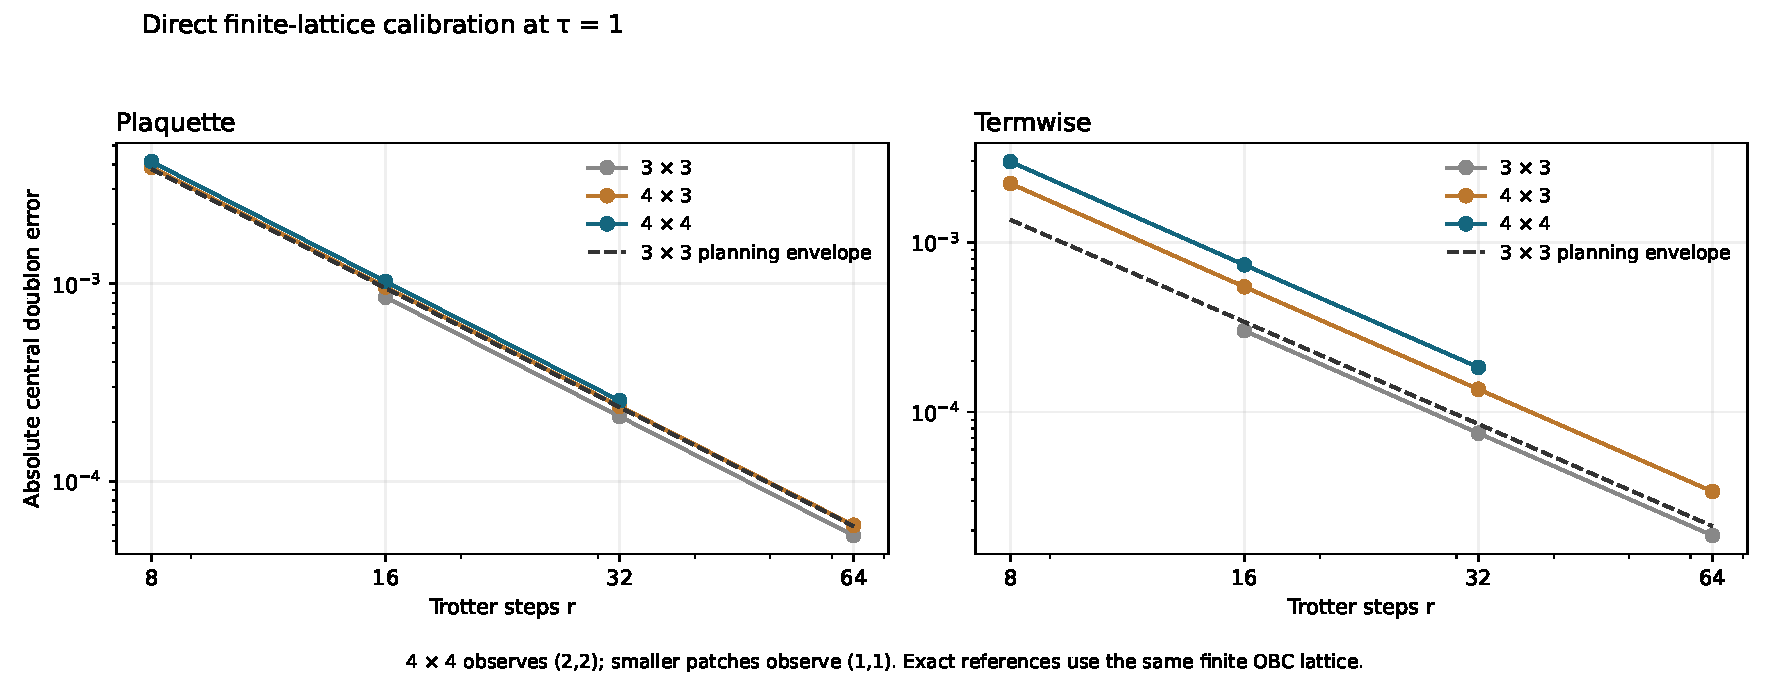
\includegraphics[width=\linewidth]{large_patch_calibration.pdf}
\caption{Direct Trotter errors at $\tau=1$ on three finite patches, with
exact references on each same lattice. Both orderings exhibit $r^{-2}$
convergence, with coefficients that depend on the patch. The dashed line
is the previous $3\times3$ planning envelope, including its $10\%$ margin.
The $4\times4$ observable is at $(2,2)$; smaller patches use $(1,1)$.
This comparison calibrates the finite $4\times4$ example and does not
certify large-$L$ or long-time transfer.}
\label{fig:large-patch}
\end{figure}

\paragraph{Longer time and the capacity sensitivity.}
We extend the same exact $4\times4$ reference and both product formulas
to $\tau=2,4$. At each time, the initial counts are $8\tau,16\tau,32\tau$;
further doubling is required if the two finest coefficients disagree by
more than $5\%$. Figure~\ref{fig:patch-time-extension} compares the converged
tails with the smaller patches. The observed site remains $(2,2)$ and
each product formula is compared with exact evolution on that same lattice.
The converged-pair coefficients on $4\times4$ are $1.096$ and $0.775$
for plaquette and termwise evolution at $\tau=2$, and $4.193$ and $3.029$
at $\tau=4$. The finest pairs agree within $0.36\%$ in all four cases.
The $\tau=4$ plaquette value is close to $4\times3$ and below $3\times3$;
the termwise value exceeds both smaller patches. A single multiplicative
finite-size correction would miss this dependence on ordering and time.

\begin{figure}[t]
\centering
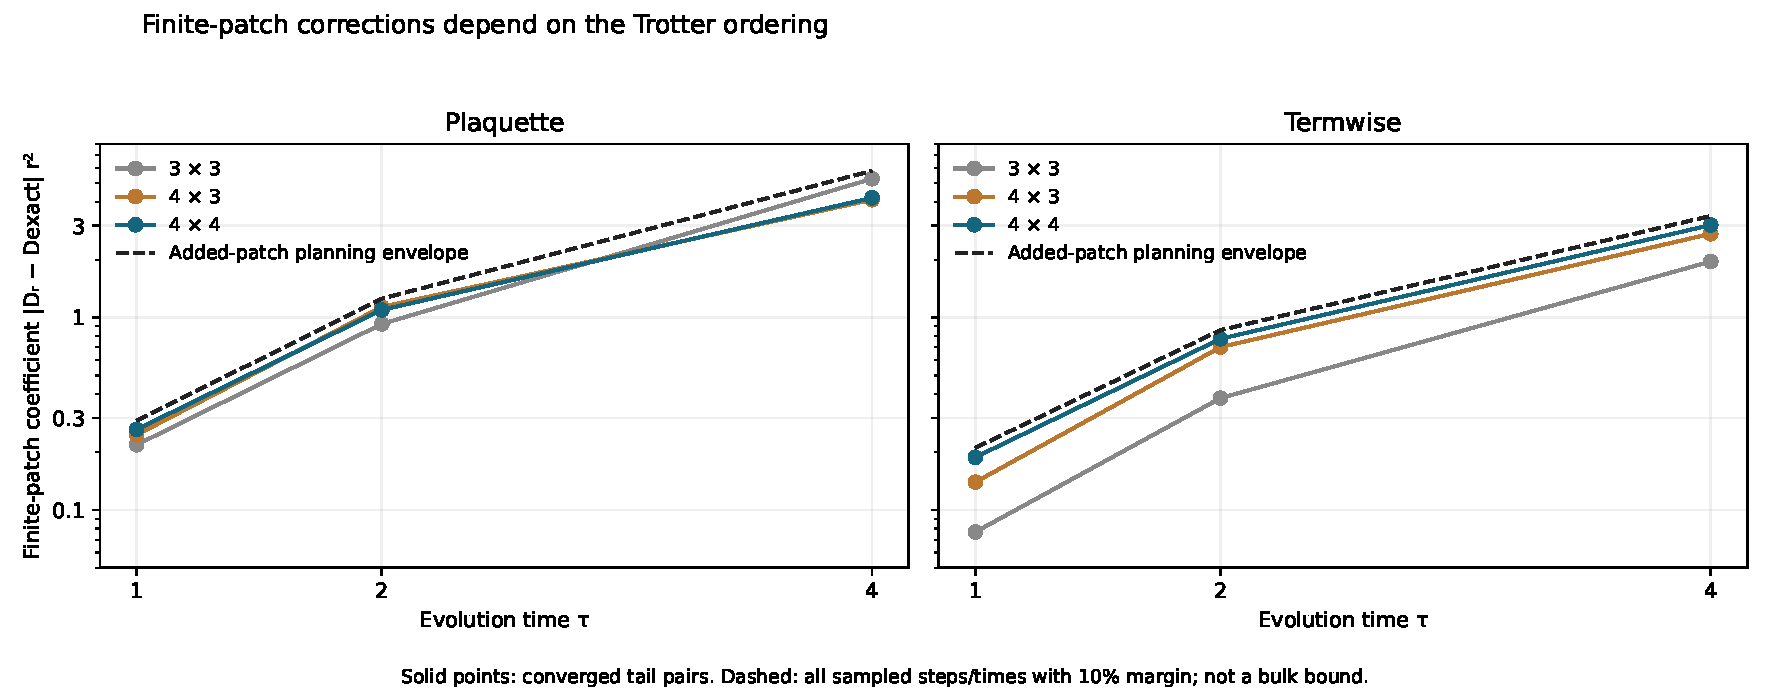
\includegraphics[width=\linewidth]{patch_time_extension.pdf}
\caption{Ordering-specific Trotter coefficients through $\tau=4$ on three
finite patches. Solid points use converged tail pairs; the dashed envelope
also covers measured coarser-step coefficients and earlier sampled times,
with a $10\%$ margin. The larger patches have only three time nodes;
unsampled time peaks and larger-lattice corrections remain possible.}
\label{fig:patch-time-extension}
\end{figure}

\subsection{Matrix-free finite-lattice reference}
Writing the state as a matrix indexed by up- and down-spin occupation masks,
we apply
\begin{equation}
 H\Psi=h_\uparrow\Psi+\Psi h_\downarrow^{\mathsf T}+V\odot\Psi.
\end{equation}
Each hopping matrix is sparse within a single spin sector; no full-sector
Hamiltonian is stored. Fermionic signs count occupied sites between the
hopping endpoints in the snake order. For $U/J=4$, the triangle bound is
$\|H\|\leq2|E|+N=64$ on $4\times4$. We evaluate
\begin{equation}
 e^{-iH\tau}\psi_0=J_0(a)\psi_0+
 2\sum_{k\geq1}(-i)^kJ_k(a)T_k(H/64)\psi_0,\qquad a=64\tau,
\end{equation}
using the three-term Chebyshev recurrence. The bound
\begin{equation}
 |J_k(a)|\leq\frac{(|a|/2)^k}{k!}
       \exp\!\left(\frac{a^2}{4(k+1)}\right)
\end{equation}
follows by bounding the absolute Bessel series; successive right-hand
sides have ratio at most $|a|/[2(k+1)]$. A geometric tail therefore selects
a degree with state truncation error below $10^{-12}$. For a $[0,1]$
observable, state error $\eta$ gives observable error at most
$2\eta+\eta^2$. This controls polynomial truncation, separately from
floating-point error. The computed $4\times4$ norm error is about
$10^{-13}$.

Trotter hopping stages use exact two-state rotations. Plaquette stages
use the fermionic Hadamard decomposition already employed by the compiler.
Complete state vectors for the exact reference and both orderings agree
with the independent Python implementation on $2\times2$, $3\times2$,
and $3\times3$ to better than $2\times10^{-11}$. Large-run outputs retain
all-site doublons, norms, input and executable hashes, and atomic case
records. The step convergence criterion is a $5\%$ agreement between the
two finest observable-error coefficients, not a proof of bulk convergence.

\section{Circuit-level calibration of the surface-code law}\label{app:surface}
We calibrate Eq.~\eqref{eq:logical} with a rotated-surface-code memory
experiment under the noise model and schedule of Table~\ref{tab:parameters}:
two-qubit depolarizing error $p$ on each CZ, one-qubit depolarizing error
$p/10$ on each Hadamard, preparation and readout flips with probability $p$,
and idle depolarizing error $p$ per unused CZ slot and per data-qubit
measurement and reset slot. Four CZ layers, a 100~ns measurement, and a
100~ns reset give the nominal 240~ns round; basis changes are fused into
the CZ slots, and their additional physical duration is not modeled.
Circuits are sampled with Stim and decoded by minimum-weight perfect matching
in PyMatching~\cite{gidney2021stim,higgott2023sparse}.

The fit uses $7.8\times10^7$ training shots at $R=10d$ and $20d$ rounds and
$1.8\times10^7$ independent holdout shots at $R=100d$, for $d=3,5,7,9$ at
$p=10^{-3}$ and $d=3,5,7$ at $p=10^{-4}$. Each basis $b\in\{X,Z\}$ has its own
amplitude and a common suppression factor,
\begin{equation}\label{eq:surface-fit}
 q_b(d)=A_b\Lambda^{-(d+1)/2},\qquad
 P_b(R)=\tfrac12\left[1-(1-2q_b)^{R+\delta_{db}}\right],
\end{equation}
where $P_b(R)$ is the probability of a logical failure after $R$ rounds and
$\delta_{db}$ absorbs preparation and readout at the endpoints. We use the
conservative sum $A=A_X+A_Z$ as the per-patch amplitude.

\begin{table}[h]
\centering
\small
\begin{tabular}{@{}rrrl@{}}
\toprule
$p$ & $\Lambda$ [95\% interval] & $A$ [95\% interval] & Note\\
\midrule
$10^{-3}$ & 7.41 [7.20, 7.62] & 0.077 [0.072, 0.083] & training fit, $d=3$--9\\
$10^{-3}$ & 7.97 [7.82, 8.11] & 0.097 [0.091, 0.103] & post hoc, $d\geq5$ at $100d$\\
$10^{-4}$ & 89 [64, 146] & 0.125 [0.062, 0.336] & $d=7$ has no observed failures\\
\bottomrule
\end{tabular}
\caption{Fitted surface-code law. Intervals are asymptotic profile-likelihood
intervals conditional on Eq.~\eqref{eq:surface-fit}.}\label{tab:surface-fit}
\end{table}

A single law is statistically rejected across $d=3$--9 at $p=10^{-3}$
(training lack of fit $p=0.013$; holdout $p=8.8\times10^{-11}$), so
Eq.~\eqref{eq:logical} is an approximate resource model rather than an exact
description. Relative to the reference $A=0.1$, $\Lambda=10$, the fitted law
raises the distance needed for $V p_L\leq\eps$ by 4--6 at $p=10^{-3}$ for
$V=10^8$--$10^{14}$ patch-rounds and $\eps=10^{-4}$--$10^{-6}$, a factor
1.3--1.5 in patch area, and by at most 2 at $p=10^{-4}$. Every such distance
lies beyond the sampled range, and lattice surgery and correlated or coherent
hardware noise are not included. The complete evidence, seeds, circuits, and
manifests are in \texttt{results/surface\_law\_v1}.


\section{STAR channels, growth, and retries}\label{app:star}
The STAR instrument of Sec.~\ref{sec:star} evaluates the transversal multi-rotation preparation exactly at every workload angle and composes it with measured growth. This appendix gives the retry structure, the accepted-channel checks, and the growth campaigns behind that model.

\subsection{Explicit retries, covariance, and parallelism}\label{sec:rus}
The logical injection instrument prepares
$|A_\theta\rangle=e^{-i\theta Z}|+\rangle$, applies
$\mathrm{CNOT}_{\mathrm{data}\to\mathrm{ancilla}}$, and measures the ancilla
in $Z$. Its data Kraus operators are
\begin{equation}
 K_0=2^{-1/2}e^{-i\theta Z},\qquad
 K_1=2^{-1/2}e^{+i\theta Z}.
\end{equation}
After outcome one, an injection of angle $2\theta$ corrects a successful
next branch: $K_0(2\theta)K_1(\theta)=K_0(\theta)/\sqrt2$.
Repeating this gives the standard angle-doubling protocol underlying the
STAR reference~\cite{akahoshi,toshio}. CUDA-Q P0 now contains explicit
preparation, CNOT, measurement, conditional retries, and a returned exhaustion
flag for caps $1,2,4,8,24$. This compilation does not supply a surface-code
injection or patch-growth implementation.

For a Pauli fault on either wire immediately before or after CNOT, each
conditional $K$ remains diagonal or antidiagonal with equal-magnitude
entries. Hence
\begin{equation}
 K^\dagger K=I/2,\qquad KZ=\pm ZK.
\end{equation}
The first identity makes the outcome probability independent of the data
state; the second makes the conditional map commute with the channel
$\mathcal Z(\rho)=Z\rho Z$. It therefore commutes with a Z-dephasing inverse,
which is a linear combination of $\mathcal I$ and $\mathcal Z$. Mixtures
of such faults and compositions over retries retain this local covariance
under the stated branch-independent Pauli model. All sixteen two-qubit
Paulis at both locations are checked independently.

This verifies the needed local commutation condition for that declared
instrument. It does not establish branch-independent residual noise for
physical state preparation, patch growth, measurement-dependent selection,
or a mismatched channel inversion. The worst-case $\Gamma q_L$ bias bound
therefore remains the default; $q_L$ is a separately labeled covariance-based
reference scenario. The physical STAR schedule still has to justify using it.

For $b$ simultaneous ideal injections with geometric success probability
$1/2$ and cap $K$, the mean batch retry time in units of one attempt is
\begin{equation}
 \mathbb E[M_b]=\sum_{k=0}^{K-1}\Pr(M_b>k)
 =\sum_{k=0}^{K-1}\left[1-(1-2^{-k})^b\right].
\end{equation}
It approaches $2$ for one lane, but is approximately $3.50$ for four lanes.
Simply dividing the serial duration by four misses the slowest retry. The
implemented policy has a barrier between batches, reserves six injection
tiles per lane, and assumes nine clocks per attempt, recovering the previous
18-clock serial mean. It forms disjoint batches using full JW supports,
not merely disjoint fermionic endpoints. An asynchronous policy could improve
this conservative batch schedule.

With $R$ rotations the ideal no-exhaustion probability is
$(1-2^{-K})^R$; the cap $K$ is chosen from a small allocated tail allowance, and
the acceptance penalty is charged.




\subsection{STAR: accepted channels and growth components}
We enumerate the projected error-angle mixture for the multirotation
construction~\cite{toshio}. For odd injection distance $d_i$, let
$k=(d_i+1)/2$ and $\alpha=\arctan(|\tan\theta|^{1/k})$. With ideal
syndrome projection, the no-fault acceptance is
\begin{equation}
 P_{\mathrm{acc}}^{(0)}=\cos^{2k}\alpha+\sin^{2k}\alpha.
\end{equation}
Independent rotation-generator Pauli faults have probability $p/15$ on
weight-two factors and $p/30$ on the final weight-one factor. Enumerating
the surviving branches gives weights $w_j$ and angle errors $\delta_j$,
with coherence multiplier $c=\sum_jw_j e^{-2i\delta_j}$. This is an exact
calculation for these faults and perfect projection; the other physical
faults of an injection circuit are not included.

Ideal probabilistic coherent-error cancellation (PCEC) composes this
channel with the conjugate mixture, giving $|c|^2$ and hence a Pauli
channel. We also execute one level of noisy PCEC in the model: sampled
inverse-angle corrections themselves use raw repeat-until-success (RUS)
channels. Their angle-dependent preparation time, retries, and growth
noise are charged. The resulting imaginary component is retained,
rather than discarded by an assumed twirl. For a histogram with rotation
multiplicities $R_j$, the separate ledger is
\begin{equation}
 \chi=-2\sum_jR_j\log(\operatorname{Re}c_j),\qquad
 B_{\mathrm{coh}}\leq\tfrac12\left[\prod_j\left(1+\frac{|\operatorname{Im}c_j|}{\operatorname{Re}c_j}\right)^{R_j}-1\right].
\end{equation}
Here $\chi$ is the dephasing-component inverse-norm estimate, while
$B_{\mathrm{coh}}$ bounds the coherent residue after that inverse; the product accounts for
its non-CPTP norm. It is not a
claim that the complete noisy gadget is Pauli. Workload retry caps reserve
1\% of $\eps$ for omitted branches; the actual aggregate tail is recorded.

Detector rejection and high-distance growth remain explicit scenarios.
We use $P_{\mathrm{acc}}=P_{\mathrm{proj}}(1-c_dp)^{d_i^2+6d_i}$, with
$c_d=1,4$, and independent growth dephasing
\begin{equation}
 f(d_i,p)=\min\!\left\{0.25,
 f_9\left(\frac{p}{10^{-3}}\right)^5\left(\frac{d_i}{9}\right)^2
 \left(\frac{0.01}{p}\right)^{-(d_i-9)/2}\right\},
 \quad f_9\in\{0,10^{-5},10^{-4}\}.
\end{equation}
There is no growth term when $d_i=d_{\mathrm{data}}=25$. The $f_9$ values are anchored at $p=10^{-3}$; their assumed extension
scales as $p^{(d_i+1)/2}$ at fixed distance. These coefficients
are not transplanted calibrations from Chung et al., whose reported noise
model differs~\cite{chung}. Switching chooses the original-injection error
reference when it is smaller after growth; its error and high-acceptance
service remain declared assumptions. The study therefore tests a mechanism
and its sensitivities, not the feasibility of a complete optimized source.

\begin{figure}[t]
\centering
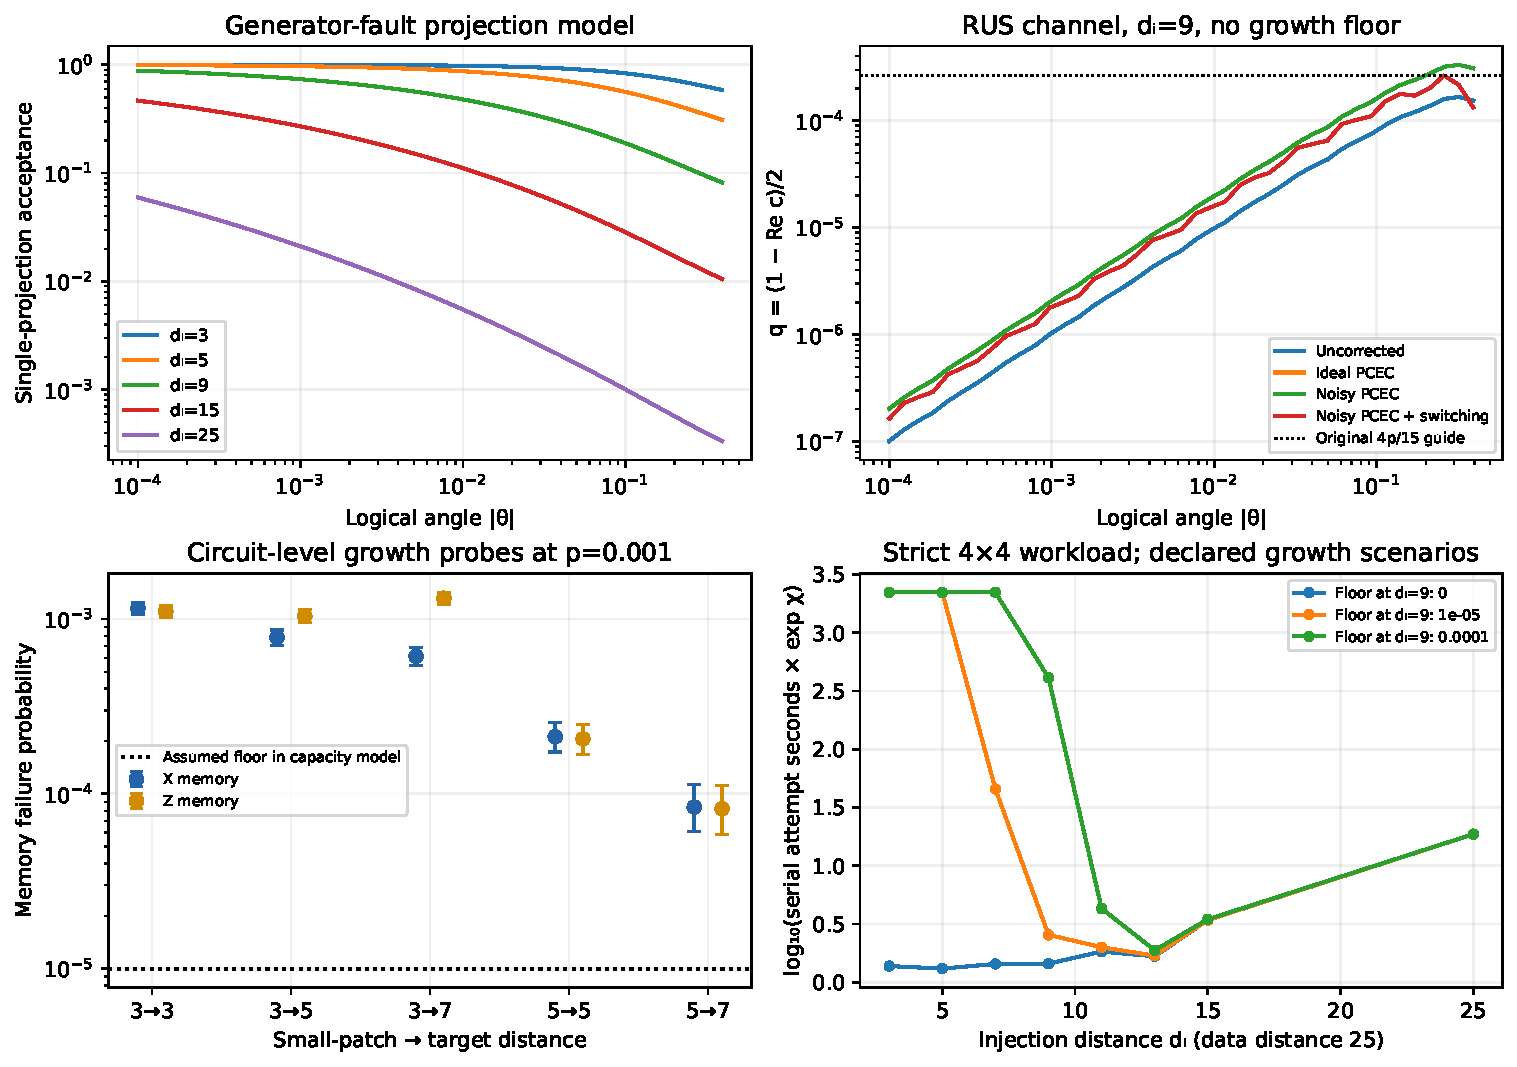
\includegraphics[width=0.94\linewidth]{implementation_star.pdf}
\caption{STAR mechanism and growth checks. Upper panels use the specified
rotation-generator fault submodel; $q=(1-\operatorname{Re}c)/2$ alone does
not describe its coherent component. Lower left: decoded X/Z memory error
for ideal small-patch preparation followed by noisy growth, stabilization,
and readout, with fixed-sample 95\% binomial intervals. The dotted floor
is a capacity-model assumption, not a fitted growth curve. Lower right:
serial service times multiplied by the dephasing sampling factor for a
fixed strict-precision $4\times4$ workload, under declared growth scenarios.
A complete injected-state error model is still required to replace the
STAR capacity assumptions.}\label{fig:implementation-star}
\end{figure}

A separate circuit-level experiment tests direct rotated-patch growth
from $d_i=3,5$ to $d_f=5,7$, with no-growth controls. The starting patch is
ideal; fresh right and bottom strips are prepared in Z and X respectively,
then the target patch is stabilized for $d_f$ rounds. Stim supplies a
nearest-neighbor extraction schedule; transition detectors are constructed
from exact stabilizer flows and later detectors compare adjacent rounds.
PyMatching decodes the circuit. Gate, reset, measurement, and idle errors
are included, with the 240\,ns cycle explicitly charged. Every one of
20 cases uses 500,000 shots, including both X/Z tests and both physical
error rates. Noiseless and deliberately inserted logical-flip controls
check that the detector and logical records are meaningful. These memory
components include final readout and exclude noisy initial injection;
they cannot establish the distance-25 arbitrary-angle growth floor.


A larger fixed-shot campaign extends the same protocol to
initial distances $d_i=5,9,13$ and final distances $d_f=13,25$ at
$p=10^{-3},10^{-4}$ in both bases. All 24 cases complete one million
shots, following a two-case PBS topology smoke. Both jobs finish with
zero exit status, and the case census retains seeds and circuit hashes.
At $p=10^{-3}$, $5\to25$ produces 51 X-basis and 419 Z-basis
failures; $5\to13$ produces 60 and 175. Every other case has zero observed
failures. A zero count has simultaneous one-sided upper bound
$6.174\times10^{-6}$ per component, using a 5\% family error budget over
all 24 intervals. If the two basis tests describe a common Pauli channel,
their union bounds its total error by $1.235\times10^{-5}$ for zero-failure
pairs. Thus these data constrain growth at the data-code distance but do
not yet certify a $10^{-5}$ total floor. They also show that the initial
patch distance matters even when the final patch is large. Initial
injection faults remain excluded, and we do not subtract the no-growth
control from a measured campaign error.


\section{Raw repeat-until-success and PCEC}\label{app:raw-rus}
At retry $m$, let the accepted rotation multiply off-diagonal elements by
$c_m=1-a_m+ib_m$ with $a_m,b_m=O(p)$. Assume independent faults between
retries, success probability exactly one half, the conjugate multiplier
$c_m^*$ on failure, and ideal angle doubling. Averaging over the RUS branches
then gives the channel multiplier
\begin{equation}\label{eq:rus-average}
 C=\sum_{n\geq0}2^{-n-1}c_n\prod_{m<n}c_m^*
 =1-\sum_{m\geq0}2^{-m}a_m+O(p^2),
\end{equation}
because the first-order coefficient of each $b_m$ is
$2^{-m-1}-\sum_{n>m}2^{-n-1}=0$. Coherence therefore cancels at first order,
while dephasing retains the weights $2^{-m}$. Ideal PCEC instead maps each
$c_m$ to $|c_m|^2$, which removes the coherent term of every trial but doubles
its dephasing to leading order.

Numerically, over 27 angles in $[10^{-3},\pi/8]$, injection distances 5, 9, and
25, and $p=10^{-3}$ and $10^{-4}$, the PCEC exposure exceeds the raw exposure
by a factor 1.999--2.007 without growth, and $|\operatorname{Im}C_{\rm raw}|$ stays
below $2.4\times10^{-7}$, falling a hundredfold when $p$ falls tenfold. With the
growth bound composed, the ratio falls to 1.5--1.6. The cancellation fails for
a biased success probability, for same-sign success and failure errors, and
for rare correlated faults; the script \texttt{python/raw\_rus\_check.py}
quantifies each case.

Toshio \textit{et al.}~\cite{toshio} average the same branches in their
Appendix~E, yet report a raw-RUS prefactor slightly larger than with PCEC and
a logarithmic dependence on the target angle. Their averaged coherent term
therefore stays first order, unlike this instrument. We have not reconciled
the conventions. Raw RUS is accordingly an option of the optimizer, charged
with its coherent residue and retry tail, rather than a conclusion that PCEC
is unnecessary. It changes the capacity leader in one of 64 cells, so the
conclusions about full fault tolerance do not depend on it; the STAR and
hybrid capacities do.


\section{Physical-qubit estimators}\label{app:nisq}
The physical arm in Fig.~\ref{fig:headline} brackets an unknown estimator
between two-qubit PEC and an assumed effective overhead. This appendix
collects the inverse problem, which states what a physical estimator would
need in order to compete, together with the compilation and noise details
behind Eq.~\eqref{eq:nisq-gates}.
\subsection{The inverse problem}
This calculation compares with the reference menu at fixed $\tau=1$ (Sec.~\ref{sec:leader}); it states
requirements on an unknown estimator and does not use the optimized encoded designs.

For a fixed physical estimator, let $F$ be its variance per attempted circuit
relative to $v_*=D_*(1-D_*)=0.09$, and let $b$ be its remaining systematic
offset. Rejection is included in $F$. At footprint $a$, attempt duration $t_a$,
and deadline $T$, the evaluation budget after training is
\begin{equation}\label{eq:nisq-attempt-budget}
 M=\max\left\{0,
 \left\lfloor\frac{Q}{a}\right\rfloor
 \left\lfloor\frac{T}{t_a}\right\rfloor-M_{\rm train}\right\}.
\end{equation}
The Gaussian planning condition and its two equivalent requirements are
\begin{align}
 e_T+b+z\sqrt{Fv_*/M}&\leq\eps,\label{eq:nisq-accuracy-requirement}\\
 F_{\max}(b,r)&=\frac{M(\eps-e_T-b)^2}{z^2v_*},\qquad
 b_{\max}(F,r)=\eps-e_T-z\sqrt{Fv_*/M},\label{eq:nisq-break-even}
\end{align}
where $z=1.96$ and $e_T=C/r^2$. An exhausted allowance is infeasible.
Figure~\ref{fig:nisq-requirements} optimizes over a declared integer-step menu;
the estimator must achieve its $F$ and $b$ at the selected $r$. We do not
assume that its overhead is independent of refinement.

\begin{figure}[!htbp]
\centering
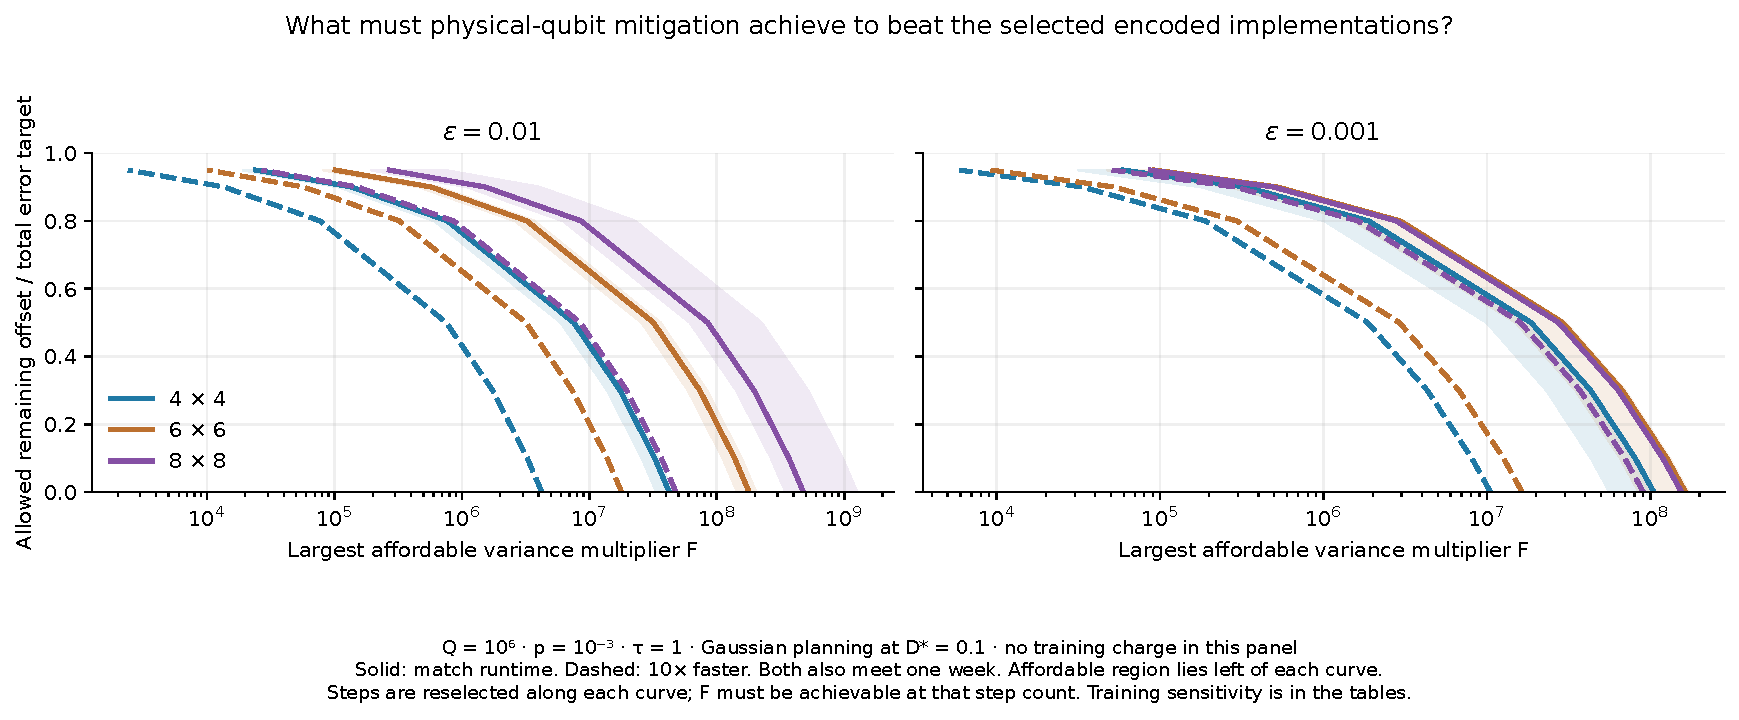
\includegraphics[width=\linewidth]{nisq_requirements.pdf}
\caption{Requirements for physical-qubit computation at $Q=10^6$, $p=10^{-3}$,
and $\tau=1$. Each curve gives the largest affordable variance multiplier as
a function of the allowed systematic offset. Solid curves match the fastest
fitting member of the selected encoded implementations; dashed curves require
a tenfold speedup. Both also meet the week cutoff. Bands span the encoded
scenarios, with steps reselected along each curve. The panel assumes zero
training charge; saved tables also charge six million training attempts.
The affordable region lies to the left of a curve. These are Gaussian planning
requirements on an unknown estimator, not predictions of an experimental
pipeline's accuracy.}\label{fig:nisq-requirements}
\end{figure}

For a requested speedup $s$, we set
$T=\min(T_{\rm week},T_{\rm encoded}/s)$, with $s=1$ or 10.
The encoded comparator is the fastest fitting member of the three selected
implementations within that scenario. Those implementations were optimized
for one-week area, not reoptimized over all allocations for runtime at this
particular $Q$. If no encoded copy fits, only the one-week physical requirement
is reported. Training uses zero or six million additional equal-duration
attempts as explicit sensitivities. A real pipeline must also account for
uncertainty in its trained correction and any shared time-series information.

For example, at $4\times4$, $Q=10^6$, and $p=10^{-3}$, allowing a
remaining offset $b=0.001$ at $\eps=0.01$ gives
$F_{\max}=3.3\times10^7$ at 13 steps, with a 67-second encoded comparator.
At $\eps=0.001$, allowing $b=10^{-4}$ gives
$F_{\max}=8.1\times10^7$ at 40 steps, with a 14-hour comparator.
These central-scenario examples charge no training. The larger affordable
multiplier in the strict case follows from the longer encoded runtime; it
does not make physical accuracy easier. An actual estimator must attain
both the stated offset and variance at the corresponding circuit depth.

The scientific decision is whether plausible accuracy and sampling costs fall
on one side of these boundaries. A detailed mitigation-transfer calculation
is most useful where resolving that question could change the ranking.
We apply the same distinction between measured components and assumed
composition to all three architectures. A capacity leader is called robust
only when its worst capacity across this scenario menu exceeds the best
capacity of both other encoded arms. Overlaps remain unresolved, and this
criterion establishes no unconditional NISQ size boundary.


\section{QUOPS model details}\label{app:quops}
\paragraph{Specification.} The benchmark definition follows the paper's
Supplementary Information: CNOT layers first, partial final layers, the
embedded polarization $\gamma=(4^wF_e-1)/(4^w-1)$ excluding terminal state
preparation and measurement, the one-sided 95\% pass rule, and the score and
rate formulas. Our model does not include the confidence margin or the SPAM
reference circuits; with $10^4$ executions the statistical margin is small.
The complete extraction, including every measured row and 27 comparisons with
another workshop implementation, is in \texttt{docs/QUOPS\_SPEC.md}.

\paragraph{Polarization.} Exact process polarizations of random circuits with
$w=2$--8 and $p=10^{-3}$--$10^{-2}$, computed by Pauli-transfer and independent
Choi calculations, agree with Eq.~\eqref{eq:quops-polarization} to 0.215\%. The
product of local gate polarizations underestimates them by factors
1.07--1.24 at mean polarization near 0.2, because a local polarization does not
account for the register dimension. Idle time lowers the polarization by 4--11\%
at odd widths 3--7.

\paragraph{Routing.} We routed 900 random circuits of widths 4--144 on the
smallest near-square grid with Cirq's RouteCQC and with a constructive
network of pair assignment, edge colouring, and row--column--row odd--even
sorting. Per benchmark layer for $16\leq w\leq144$, RouteCQC needs
$0.071w^{1.68}$ added SWAPs and $0.35w^{1.59}$ fused two-qubit gates, with
two-qubit depth growing as $w^{1.04}$; the constructive network needs about
three times more gates but its depth grows only as $w^{0.62}$. Doubling the
available area changed no cost under the tested placement. The model uses the
measured means through $w=144$, the fits beyond, and the router with smaller
polarization loss at each width.

\paragraph{Encoded arms.} Each layer of long-range CNOTs is assumed to take two
code clocks by lattice surgery in the fast block, without congestion; this is
the least tested assumption for large widths. STAR averages its injection
instrument over the wrapped angles with sixteen samples. FT splits the loss
budget between synthesis, magic states, and logical faults on a declared grid
and optimizes ports, factories up to 4096, cleanup, and distance.


\section{Fixed-time benchmark}\label{app:fixed-tau}
Figure~\ref{fig:optimization-fixed-tau} repeats the capacity comparison at
fixed $\tau=1$. Beyond $L\approx8$ it compares the cost of evolving full
lattices rather than the accuracy of a local answer, which is why the main
text leads with $\tau=L/4$. The ordering is the same, with larger analog
gains: at $p=10^{-3}$, $\eps=0.01$, and $10^8$ qubits, STAR reaches
$L=16$ and the hybrid $L=24$, compared with 12 and 16 under the reference menu.

\begin{figure}[h]
\centering
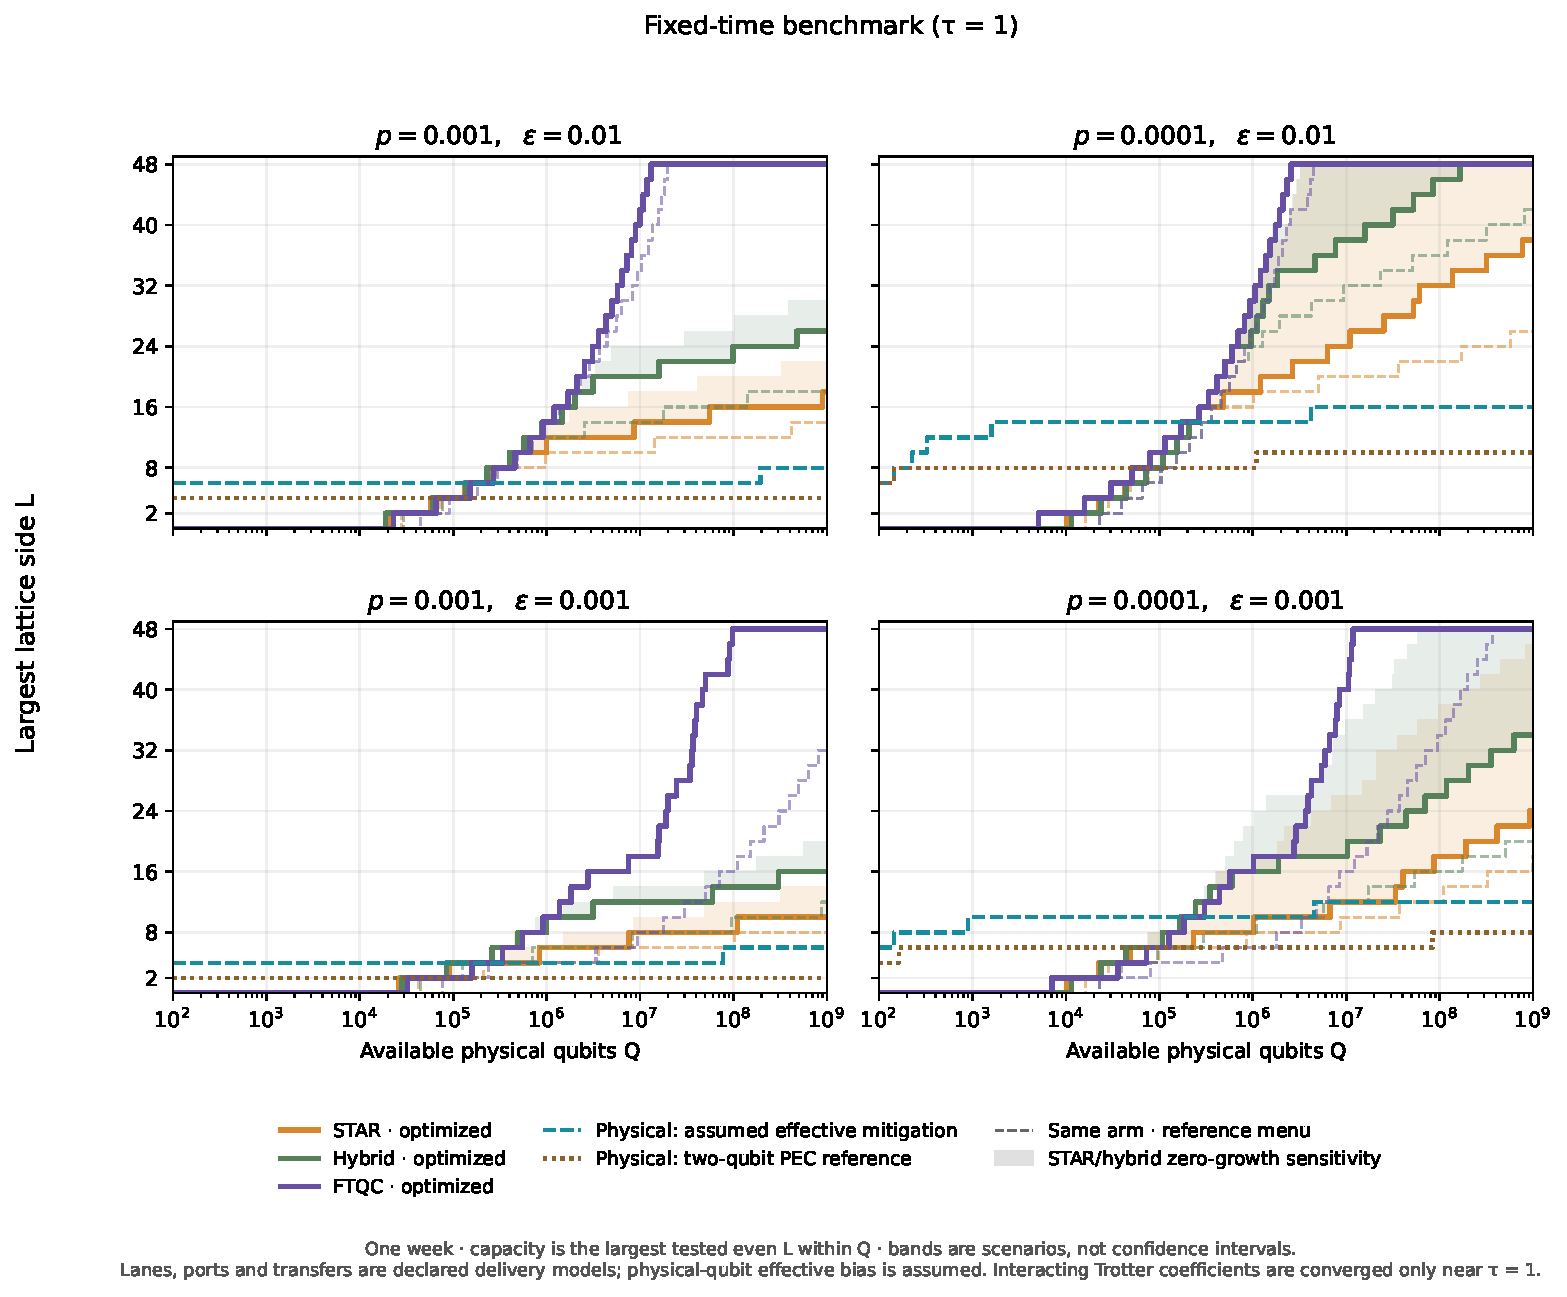
\includegraphics[width=\linewidth]{optimization_round_fixed_tau_v2.pdf}
\caption{Fixed-time benchmark at $\tau=1$, drawn as in Fig.~\ref{fig:headline}.
Beyond $L\approx8$ these curves compare the cost of evolving full lattices, not
the accuracy of a local answer.}\label{fig:optimization-fixed-tau}
\end{figure}


\section{Reproducibility}\label{app:reproducibility}
Every number in the main text is regenerated from saved results by the repository's \texttt{Makefile}: \texttt{make optimization-round-v2-figures} and \texttt{make quops-figures} redraw the capability figures, and \texttt{make audit} replays every saved calculation against its declared inputs, including the surface-code calibration, the raw-RUS checks, and the two optimization rounds. The sweeps themselves run on a compute node with \texttt{pbs/optimization\_round.pbs} and \texttt{python/quops\_study.py}. The Supplementary Material preserves the development history, earlier reference models, and compilation checks.

\bibliographystyle{unsrt}
\bibliography{references}
\end{document}
